% Options for packages loaded elsewhere
\PassOptionsToPackage{unicode}{hyperref}
\PassOptionsToPackage{hyphens}{url}
\PassOptionsToPackage{dvipsnames,svgnames,x11names}{xcolor}
%
\documentclass[
  11pt,
  letterpaper,
  DIV=11,
  numbers=noendperiod]{scrartcl}

\usepackage{amsmath,amssymb}
\usepackage{iftex}
\ifPDFTeX
  \usepackage[T1]{fontenc}
  \usepackage[utf8]{inputenc}
  \usepackage{textcomp} % provide euro and other symbols
\else % if luatex or xetex
  \usepackage{unicode-math}
  \defaultfontfeatures{Scale=MatchLowercase}
  \defaultfontfeatures[\rmfamily]{Ligatures=TeX,Scale=1}
\fi
\usepackage{lmodern}
\ifPDFTeX\else  
    % xetex/luatex font selection
\fi
% Use upquote if available, for straight quotes in verbatim environments
\IfFileExists{upquote.sty}{\usepackage{upquote}}{}
\IfFileExists{microtype.sty}{% use microtype if available
  \usepackage[]{microtype}
  \UseMicrotypeSet[protrusion]{basicmath} % disable protrusion for tt fonts
}{}
\makeatletter
\@ifundefined{KOMAClassName}{% if non-KOMA class
  \IfFileExists{parskip.sty}{%
    \usepackage{parskip}
  }{% else
    \setlength{\parindent}{0pt}
    \setlength{\parskip}{6pt plus 2pt minus 1pt}}
}{% if KOMA class
  \KOMAoptions{parskip=half}}
\makeatother
\usepackage{xcolor}
\setlength{\emergencystretch}{3em} % prevent overfull lines
\setcounter{secnumdepth}{-\maxdimen} % remove section numbering
% Make \paragraph and \subparagraph free-standing
\ifx\paragraph\undefined\else
  \let\oldparagraph\paragraph
  \renewcommand{\paragraph}[1]{\oldparagraph{#1}\mbox{}}
\fi
\ifx\subparagraph\undefined\else
  \let\oldsubparagraph\subparagraph
  \renewcommand{\subparagraph}[1]{\oldsubparagraph{#1}\mbox{}}
\fi

\usepackage{color}
\usepackage{fancyvrb}
\newcommand{\VerbBar}{|}
\newcommand{\VERB}{\Verb[commandchars=\\\{\}]}
\DefineVerbatimEnvironment{Highlighting}{Verbatim}{commandchars=\\\{\}}
% Add ',fontsize=\small' for more characters per line
\usepackage{framed}
\definecolor{shadecolor}{RGB}{241,243,245}
\newenvironment{Shaded}{\begin{snugshade}}{\end{snugshade}}
\newcommand{\AlertTok}[1]{\textcolor[rgb]{0.68,0.00,0.00}{#1}}
\newcommand{\AnnotationTok}[1]{\textcolor[rgb]{0.37,0.37,0.37}{#1}}
\newcommand{\AttributeTok}[1]{\textcolor[rgb]{0.40,0.45,0.13}{#1}}
\newcommand{\BaseNTok}[1]{\textcolor[rgb]{0.68,0.00,0.00}{#1}}
\newcommand{\BuiltInTok}[1]{\textcolor[rgb]{0.00,0.23,0.31}{#1}}
\newcommand{\CharTok}[1]{\textcolor[rgb]{0.13,0.47,0.30}{#1}}
\newcommand{\CommentTok}[1]{\textcolor[rgb]{0.37,0.37,0.37}{#1}}
\newcommand{\CommentVarTok}[1]{\textcolor[rgb]{0.37,0.37,0.37}{\textit{#1}}}
\newcommand{\ConstantTok}[1]{\textcolor[rgb]{0.56,0.35,0.01}{#1}}
\newcommand{\ControlFlowTok}[1]{\textcolor[rgb]{0.00,0.23,0.31}{#1}}
\newcommand{\DataTypeTok}[1]{\textcolor[rgb]{0.68,0.00,0.00}{#1}}
\newcommand{\DecValTok}[1]{\textcolor[rgb]{0.68,0.00,0.00}{#1}}
\newcommand{\DocumentationTok}[1]{\textcolor[rgb]{0.37,0.37,0.37}{\textit{#1}}}
\newcommand{\ErrorTok}[1]{\textcolor[rgb]{0.68,0.00,0.00}{#1}}
\newcommand{\ExtensionTok}[1]{\textcolor[rgb]{0.00,0.23,0.31}{#1}}
\newcommand{\FloatTok}[1]{\textcolor[rgb]{0.68,0.00,0.00}{#1}}
\newcommand{\FunctionTok}[1]{\textcolor[rgb]{0.28,0.35,0.67}{#1}}
\newcommand{\ImportTok}[1]{\textcolor[rgb]{0.00,0.46,0.62}{#1}}
\newcommand{\InformationTok}[1]{\textcolor[rgb]{0.37,0.37,0.37}{#1}}
\newcommand{\KeywordTok}[1]{\textcolor[rgb]{0.00,0.23,0.31}{#1}}
\newcommand{\NormalTok}[1]{\textcolor[rgb]{0.00,0.23,0.31}{#1}}
\newcommand{\OperatorTok}[1]{\textcolor[rgb]{0.37,0.37,0.37}{#1}}
\newcommand{\OtherTok}[1]{\textcolor[rgb]{0.00,0.23,0.31}{#1}}
\newcommand{\PreprocessorTok}[1]{\textcolor[rgb]{0.68,0.00,0.00}{#1}}
\newcommand{\RegionMarkerTok}[1]{\textcolor[rgb]{0.00,0.23,0.31}{#1}}
\newcommand{\SpecialCharTok}[1]{\textcolor[rgb]{0.37,0.37,0.37}{#1}}
\newcommand{\SpecialStringTok}[1]{\textcolor[rgb]{0.13,0.47,0.30}{#1}}
\newcommand{\StringTok}[1]{\textcolor[rgb]{0.13,0.47,0.30}{#1}}
\newcommand{\VariableTok}[1]{\textcolor[rgb]{0.07,0.07,0.07}{#1}}
\newcommand{\VerbatimStringTok}[1]{\textcolor[rgb]{0.13,0.47,0.30}{#1}}
\newcommand{\WarningTok}[1]{\textcolor[rgb]{0.37,0.37,0.37}{\textit{#1}}}

\providecommand{\tightlist}{%
  \setlength{\itemsep}{0pt}\setlength{\parskip}{0pt}}\usepackage{longtable,booktabs,array}
\usepackage{calc} % for calculating minipage widths
% Correct order of tables after \paragraph or \subparagraph
\usepackage{etoolbox}
\makeatletter
\patchcmd\longtable{\par}{\if@noskipsec\mbox{}\fi\par}{}{}
\makeatother
% Allow footnotes in longtable head/foot
\IfFileExists{footnotehyper.sty}{\usepackage{footnotehyper}}{\usepackage{footnote}}
\makesavenoteenv{longtable}
\usepackage{graphicx}
\makeatletter
\def\maxwidth{\ifdim\Gin@nat@width>\linewidth\linewidth\else\Gin@nat@width\fi}
\def\maxheight{\ifdim\Gin@nat@height>\textheight\textheight\else\Gin@nat@height\fi}
\makeatother
% Scale images if necessary, so that they will not overflow the page
% margins by default, and it is still possible to overwrite the defaults
% using explicit options in \includegraphics[width, height, ...]{}
\setkeys{Gin}{width=\maxwidth,height=\maxheight,keepaspectratio}
% Set default figure placement to htbp
\makeatletter
\def\fps@figure{htbp}
\makeatother

\usepackage{authblk}
\renewcommand\Authfont{\normalsize}
\renewcommand\Affilfont{\itshape\small}
\setlength{\affilsep}{0.5em}
\pagestyle{plain}
\KOMAoption{captions}{tableheading}
\makeatletter
\@ifpackageloaded{caption}{}{\usepackage{caption}}
\AtBeginDocument{%
\ifdefined\contentsname
  \renewcommand*\contentsname{Table of contents}
\else
  \newcommand\contentsname{Table of contents}
\fi
\ifdefined\listfigurename
  \renewcommand*\listfigurename{List of Figures}
\else
  \newcommand\listfigurename{List of Figures}
\fi
\ifdefined\listtablename
  \renewcommand*\listtablename{List of Tables}
\else
  \newcommand\listtablename{List of Tables}
\fi
\ifdefined\figurename
  \renewcommand*\figurename{Figure}
\else
  \newcommand\figurename{Figure}
\fi
\ifdefined\tablename
  \renewcommand*\tablename{Table}
\else
  \newcommand\tablename{Table}
\fi
}
\@ifpackageloaded{float}{}{\usepackage{float}}
\floatstyle{ruled}
\@ifundefined{c@chapter}{\newfloat{codelisting}{h}{lop}}{\newfloat{codelisting}{h}{lop}[chapter]}
\floatname{codelisting}{Listing}
\newcommand*\listoflistings{\listof{codelisting}{List of Listings}}
\makeatother
\makeatletter
\makeatother
\makeatletter
\@ifpackageloaded{caption}{}{\usepackage{caption}}
\@ifpackageloaded{subcaption}{}{\usepackage{subcaption}}
\makeatother
\ifLuaTeX
  \usepackage{selnolig}  % disable illegal ligatures
\fi
\usepackage{bookmark}

\IfFileExists{xurl.sty}{\usepackage{xurl}}{} % add URL line breaks if available
\urlstyle{same} % disable monospaced font for URLs
\hypersetup{
  pdftitle={Supplementary Information: Disrupting the Dichotomy between Compact and Low-Density Urbanism in the Archaeological Record},
  colorlinks=true,
  linkcolor={blue},
  filecolor={Maroon},
  citecolor={Blue},
  urlcolor={Blue},
  pdfcreator={LaTeX via pandoc}}

\title{Supplementary Information: Disrupting the Dichotomy between
Compact and Low-Density Urbanism in the Archaeological Record}
\author{}
\date{2025-05-02}

\begin{document}
\maketitle

\textbf{W. Christopher Carleton¹}, \textbf{Sarah Klassen²}, \textbf{John
T. Murphy³}, \textbf{Patrick Roberts¹}

¹ \emph{Department of Coevolution of Land Use and Urbanisation, Max
Planck Institute of Geoanthropology, Jena, Germany} ² \emph{Center for
Collaborative Synthesis in Archaeology, University of Colorado, Boulder,
Colorado, USA}\\
³ \emph{Department of Anthropology, Northern Illinois University,
Dekalb, Illinois, USA}

emails: carleton@gea.mpg.de, sarah.klassen@colorado.edu,
jmurphy7@niu.edu, roberts@gea.mpg.de

\subsection{Overview}\label{overview}

This computational notebook contains the code necessary to rerun the
analyses described in the associated paper. In order to gather and
prepare the data used in this notebook for the Hampshire case, run the
other computational notebook in the same folder (``doomsday.ipynb'')
first. Then, run all of the following code in order.

\subsection{Set Up}\label{set-up}

\subsubsection{Libraries}\label{libraries}

\begin{Shaded}
\begin{Highlighting}[]
\CommentTok{\# core}
\ImportTok{import}\NormalTok{ numpy }\ImportTok{as}\NormalTok{ np}
\ImportTok{import}\NormalTok{ pandas }\ImportTok{as}\NormalTok{ pd}
\ImportTok{from}\NormalTok{ scipy.stats }\ImportTok{import}\NormalTok{ norm}
\ImportTok{import}\NormalTok{ warnings}

\CommentTok{\# Plotting}
\ImportTok{import}\NormalTok{ matplotlib }\ImportTok{as}\NormalTok{ mpl}
\ImportTok{import}\NormalTok{ matplotlib.pyplot }\ImportTok{as}\NormalTok{ plt}
\ImportTok{import}\NormalTok{ seaborn }\ImportTok{as}\NormalTok{ sns}
\ImportTok{import}\NormalTok{ contextily }\ImportTok{as}\NormalTok{ ctx}

\CommentTok{\# chronocluster}
\ImportTok{from}\NormalTok{ chronocluster }\ImportTok{import}\NormalTok{ clustering}
\ImportTok{from}\NormalTok{ chronocluster.utils }\ImportTok{import}\NormalTok{ (}
\NormalTok{    clustering\_heatmap, }
\NormalTok{    pdiff\_heatmap, }
\NormalTok{    get\_box, }
\NormalTok{    chrono\_plot, }
\NormalTok{    chrono\_plot2d, }
\NormalTok{    inclusion\_legend}
\NormalTok{)}
\ImportTok{from}\NormalTok{ chronocluster.distributions }\ImportTok{import}\NormalTok{ ddelta}
\end{Highlighting}
\end{Shaded}

\subsubsection{Plot Styling}\label{plot-styling}

\begin{Shaded}
\begin{Highlighting}[]
\CommentTok{\# basic styling}
\NormalTok{plt.style.use(}\StringTok{\textquotesingle{}ggplot\textquotesingle{}}\NormalTok{)}
\NormalTok{sns.set\_context(}\StringTok{"paper"}\NormalTok{)}

\CommentTok{\# matplotlib fonts}
\NormalTok{mpl.rcParams[}\StringTok{"font.size"}\NormalTok{] }\OperatorTok{=} \DecValTok{12}
\NormalTok{mpl.rcParams[}\StringTok{"legend.frameon"}\NormalTok{] }\OperatorTok{=} \VariableTok{False}
\NormalTok{mpl.rcParams[}\StringTok{"legend.fontsize"}\NormalTok{] }\OperatorTok{=} \DecValTok{10}
\NormalTok{mpl.rcParams[}\StringTok{"axes.labelsize"}\NormalTok{] }\OperatorTok{=} \DecValTok{12}
\NormalTok{mpl.rcParams[}\StringTok{"axes.titlesize"}\NormalTok{] }\OperatorTok{=} \DecValTok{14}
\NormalTok{mpl.rcParams[}\StringTok{\textquotesingle{}figure.facecolor\textquotesingle{}}\NormalTok{] }\OperatorTok{=} \StringTok{\textquotesingle{}white\textquotesingle{}}
\end{Highlighting}
\end{Shaded}

\subsubsection{NOTE: Warnings}\label{note-warnings}

Some of the plotting workarounds have generated immaterial warnings
below. In order to avoid these showing up in a PDF or HTML version of
this notebook, like the one that will be subimitted as SI alongside the
associated paper, run the next cell. In order to see the warnings,
remove the cell or change plot\_warnings to True.

\begin{Shaded}
\begin{Highlighting}[]
\NormalTok{plot\_warnings }\OperatorTok{=} \VariableTok{False}
\ControlFlowTok{if} \KeywordTok{not}\NormalTok{ plot\_warnings:}
\NormalTok{    warnings.filterwarnings(}\StringTok{"ignore"}\NormalTok{)}
\end{Highlighting}
\end{Shaded}

\subsection{Angkor}\label{angkor}

\subsubsection{Data Wrangling}\label{data-wrangling}

\begin{Shaded}
\begin{Highlighting}[]
\CommentTok{\# data wrangling}
\NormalTok{df }\OperatorTok{=}\NormalTok{ pd.read\_csv(}\StringTok{\textquotesingle{}../Data/temples\_with\_predicted\_ages.csv\textquotesingle{}}\NormalTok{)}
\NormalTok{df }\OperatorTok{=}\NormalTok{ df.dropna(subset}\OperatorTok{=}\NormalTok{[}\StringTok{\textquotesingle{}xeast\textquotesingle{}}\NormalTok{, }\StringTok{\textquotesingle{}ynorth\textquotesingle{}}\NormalTok{, }\StringTok{\textquotesingle{}model\_age\_mean\textquotesingle{}}\NormalTok{])}
\end{Highlighting}
\end{Shaded}

\paragraph{Create Points List}\label{create-points-list}

\begin{Shaded}
\begin{Highlighting}[]
\NormalTok{points }\OperatorTok{=}\NormalTok{ [}
\NormalTok{    clustering.Point(}
\NormalTok{        x}\OperatorTok{=}\NormalTok{row[}\StringTok{\textquotesingle{}xeast\textquotesingle{}}\NormalTok{],}
\NormalTok{        y}\OperatorTok{=}\NormalTok{row[}\StringTok{\textquotesingle{}ynorth\textquotesingle{}}\NormalTok{],}
\NormalTok{        start\_distribution }\OperatorTok{=}\NormalTok{ (}
\NormalTok{            ddelta(d}\OperatorTok{=}\NormalTok{row[}\StringTok{\textquotesingle{}model\_age\_mean\textquotesingle{}}\NormalTok{]) }
            \ControlFlowTok{if}\NormalTok{ row[}\StringTok{\textquotesingle{}model\_age\_sd\textquotesingle{}}\NormalTok{] }\OperatorTok{==} \DecValTok{0} 
            \ControlFlowTok{else}\NormalTok{ norm(loc}\OperatorTok{=}\NormalTok{row[}\StringTok{\textquotesingle{}model\_age\_mean\textquotesingle{}}\NormalTok{], scale}\OperatorTok{=}\NormalTok{row[}\StringTok{\textquotesingle{}model\_age\_sd\textquotesingle{}}\NormalTok{])}
\NormalTok{            ),}
\NormalTok{        end\_distribution }\OperatorTok{=}\NormalTok{ ddelta(}\DecValTok{1500}\NormalTok{)}
\NormalTok{    )}
    \ControlFlowTok{for}\NormalTok{ \_, row }\KeywordTok{in}\NormalTok{ df.iterrows()}
\NormalTok{]}

\CommentTok{\# just double check the first ten look right}
\NormalTok{points[:}\DecValTok{10}\NormalTok{]}
\NormalTok{angkor\_points }\OperatorTok{=}\NormalTok{ points}
\end{Highlighting}
\end{Shaded}

\paragraph{Figure S1: Spacetime Volume of Angkor's
Temples}\label{figure-s1-spacetime-volume-of-angkors-temples}

\begin{Shaded}
\begin{Highlighting}[]
\CommentTok{\# Custom styling parameters}
\NormalTok{style\_params }\OperatorTok{=}\NormalTok{ \{}
    \StringTok{\textquotesingle{}start\_mean\_color\textquotesingle{}}\NormalTok{: }\VariableTok{None}\NormalTok{,  }\CommentTok{\# Do not plot start mean points}
    \StringTok{\textquotesingle{}end\_mean\_color\textquotesingle{}}\NormalTok{: }\VariableTok{None}\NormalTok{, }\CommentTok{\# Do not plot end mean points}
    \StringTok{\textquotesingle{}mean\_point\_size\textquotesingle{}}\NormalTok{: }\DecValTok{10}\NormalTok{,}
    \StringTok{\textquotesingle{}cylinder\_color\textquotesingle{}}\NormalTok{: (}\FloatTok{0.3}\NormalTok{, }\FloatTok{0.3}\NormalTok{, }\FloatTok{0.3}\NormalTok{),  }\CommentTok{\# Dark grey}
    \StringTok{\textquotesingle{}ppf\_limits\textquotesingle{}}\NormalTok{: (}\FloatTok{0.05}\NormalTok{, }\FloatTok{0.95}\NormalTok{),  }\CommentTok{\# Use different ppf limits}
    \StringTok{\textquotesingle{}shadow\_color\textquotesingle{}}\NormalTok{: (}\FloatTok{0.4}\NormalTok{, }\FloatTok{0.4}\NormalTok{, }\FloatTok{0.4}\NormalTok{),  }\CommentTok{\# grey}
    \StringTok{\textquotesingle{}shadow\_size\textquotesingle{}}\NormalTok{: }\DecValTok{10}\NormalTok{,}
    \StringTok{\textquotesingle{}time\_slice\_color\textquotesingle{}}\NormalTok{: (}\FloatTok{0.5}\NormalTok{, }\FloatTok{0.5}\NormalTok{, }\FloatTok{0.5}\NormalTok{),  }\CommentTok{\# Grey}
    \StringTok{\textquotesingle{}time\_slice\_alpha\textquotesingle{}}\NormalTok{: }\FloatTok{0.3}\NormalTok{,}
    \StringTok{\textquotesingle{}time\_slice\_point\_color\textquotesingle{}}\NormalTok{: (}\DecValTok{0}\NormalTok{, }\DecValTok{0}\NormalTok{, }\DecValTok{0}\NormalTok{),  }\CommentTok{\# Black}
\NormalTok{\}}

\CommentTok{\# Plot the points using the chrono\_plot function with custom styling and a }
\CommentTok{\# time slice plane}
\NormalTok{ax\_stv\_angkor, fig\_stv\_angkor }\OperatorTok{=}\NormalTok{ chrono\_plot(points, }
\NormalTok{                                            style\_params}\OperatorTok{=}\NormalTok{style\_params, }
\NormalTok{                                            time\_slice}\OperatorTok{=}\DecValTok{1000}\NormalTok{,}
\NormalTok{                                            title}\OperatorTok{=}\StringTok{\textquotesingle{}Angkor\textquotesingle{}}\NormalTok{)}
\NormalTok{ax\_stv\_angkor.set\_box\_aspect(}\VariableTok{None}\NormalTok{, zoom}\OperatorTok{=}\FloatTok{0.85}\NormalTok{)}
\NormalTok{plt.savefig(}\StringTok{"../Output/spacetime\_volume\_Angkor.svg"}\NormalTok{, bbox\_inches}\OperatorTok{=}\StringTok{\textquotesingle{}tight\textquotesingle{}}\NormalTok{) }
\end{Highlighting}
\end{Shaded}

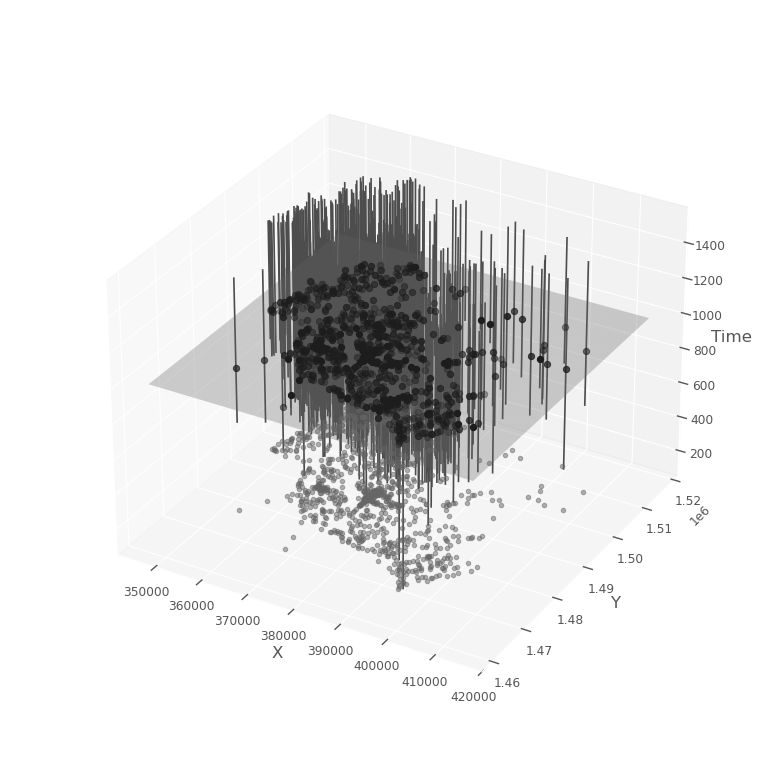
\includegraphics{analysis_files/figure-pdf/cell-7-output-1.png}

\paragraph{Define Time Slices}\label{define-time-slices}

\begin{Shaded}
\begin{Highlighting}[]
\CommentTok{\# Define the time slices}
\NormalTok{start\_time }\OperatorTok{=} \DecValTok{800}
\NormalTok{end\_time }\OperatorTok{=} \DecValTok{1200}
\NormalTok{time\_interval }\OperatorTok{=} \DecValTok{50}
\NormalTok{time\_slices }\OperatorTok{=}\NormalTok{ np.arange(start\_time, end\_time, time\_interval)}
\NormalTok{time\_slices}
\end{Highlighting}
\end{Shaded}

\begin{verbatim}
array([ 800,  850,  900,  950, 1000, 1050, 1100, 1150])
\end{verbatim}

\paragraph{GPU Boosted Pairwise Distance Density
KDEs}\label{gpu-boosted-pairwise-distance-density-kdes}

\begin{Shaded}
\begin{Highlighting}[]
\ImportTok{from}\NormalTok{ cuml.neighbors }\ImportTok{import}\NormalTok{ KernelDensity}

\KeywordTok{def}\NormalTok{ cuml\_kde(distances, bandwidth, }\OperatorTok{**}\NormalTok{kwargs):}
\NormalTok{    distances }\OperatorTok{=}\NormalTok{ np.array(distances).reshape(}\OperatorTok{{-}}\DecValTok{1}\NormalTok{, }\DecValTok{1}\NormalTok{)}

    \ControlFlowTok{if}\NormalTok{ bandwidth }\KeywordTok{is} \VariableTok{None}\NormalTok{:}
\NormalTok{        n }\OperatorTok{=} \BuiltInTok{len}\NormalTok{(distances)}
        \ControlFlowTok{if}\NormalTok{ n }\OperatorTok{\textless{}} \DecValTok{2}\NormalTok{:}
            \ControlFlowTok{raise} \PreprocessorTok{ValueError}\NormalTok{(}
                \StringTok{"Data must contain at least 2 points "}\NormalTok{, }
                \StringTok{"for bandwidth calculation."}
\NormalTok{            )}
\NormalTok{        std\_dev }\OperatorTok{=}\NormalTok{ np.std(distances, ddof}\OperatorTok{=}\DecValTok{1}\NormalTok{)}
\NormalTok{        bandwidth }\OperatorTok{=}\NormalTok{ std\_dev }\OperatorTok{*}\NormalTok{ n }\OperatorTok{**}\NormalTok{ (}\OperatorTok{{-}}\DecValTok{1} \OperatorTok{/} \DecValTok{5}\NormalTok{)}
    
\NormalTok{    kde }\OperatorTok{=}\NormalTok{ KernelDensity(kernel}\OperatorTok{=}\StringTok{"gaussian"}\NormalTok{, bandwidth}\OperatorTok{=}\NormalTok{bandwidth, }\OperatorTok{**}\NormalTok{kwargs)}
\NormalTok{    kde.fit(distances)}

    \KeywordTok{def}\NormalTok{ kde\_function(points):}
\NormalTok{        points }\OperatorTok{=}\NormalTok{ np.array(points).reshape(}\OperatorTok{{-}}\DecValTok{1}\NormalTok{, }\DecValTok{1}\NormalTok{)}
        \CommentTok{\# score\_samples returns a cupy array; use .get() to convert to NumPy}
        \ControlFlowTok{return}\NormalTok{ np.exp(kde.score\_samples(points).get())}
    
    \ControlFlowTok{return}\NormalTok{ kde\_function}
\end{Highlighting}
\end{Shaded}

\paragraph{Figure S2: Heatmap of Pairwise Distance Density versus Time
at
Angkor}\label{figure-s2-heatmap-of-pairwise-distance-density-versus-time-at-angkor}

\begin{Shaded}
\begin{Highlighting}[]
\CommentTok{\# Run the Monte Carlo simulation to get an ensemble of probable }
\CommentTok{\# lists of points included in each time slice.}
\NormalTok{num\_iterations }\OperatorTok{=} \DecValTok{500}
\NormalTok{simulations\_angkor }\OperatorTok{=}\NormalTok{ clustering.mc\_samples(}
\NormalTok{    points, }
\NormalTok{    time\_slices}\OperatorTok{=}\NormalTok{time\_slices,  }
\NormalTok{    num\_iterations}\OperatorTok{=}\NormalTok{num\_iterations}
\NormalTok{)}

\CommentTok{\# Get a bounding box for use later and to extract sensible distance limits}
\NormalTok{x\_min, y\_min, x\_max, y\_max }\OperatorTok{=}\NormalTok{ get\_box(points)}
\NormalTok{max\_distance }\OperatorTok{=}\NormalTok{ np.ceil(np.sqrt((x\_max }\OperatorTok{{-}}\NormalTok{ x\_min)}\OperatorTok{**}\DecValTok{2} \OperatorTok{+}\NormalTok{ (y\_max }\OperatorTok{{-}}\NormalTok{ y\_min)}\OperatorTok{**}\DecValTok{2}\NormalTok{))}

\CommentTok{\# set consistent pairwise bandwidth (binning of distances)}
\NormalTok{use\_kde }\OperatorTok{=} \VariableTok{True}
\NormalTok{pair\_bw }\OperatorTok{=} \VariableTok{None}
\NormalTok{kde\_sample\_n }\OperatorTok{=} \DecValTok{50}
\NormalTok{kde\_custom}\OperatorTok{=}\NormalTok{cuml\_kde}

\CommentTok{\# Produce pairwise distances to explore clustering structure}
\NormalTok{pairwise\_density\_angkor, support\_angkor }\OperatorTok{=}\NormalTok{ clustering.temporal\_pairwise(}
\NormalTok{    simulations\_angkor, }
\NormalTok{    time\_slices,}
\NormalTok{    bw}\OperatorTok{=}\NormalTok{pair\_bw, }
\NormalTok{    use\_kde}\OperatorTok{=}\NormalTok{use\_kde, }
\NormalTok{    kde\_sample\_n}\OperatorTok{=}\NormalTok{kde\_sample\_n,}
\NormalTok{    max\_distance}\OperatorTok{=}\NormalTok{max\_distance,}
\NormalTok{    kde\_custom}\OperatorTok{=}\NormalTok{kde\_custom}
\NormalTok{)}

\CommentTok{\# Visualize clustering with heatmap}
\NormalTok{clustering\_heatmap(}
\NormalTok{    pairwise\_density\_angkor,}
\NormalTok{    support\_angkor,}
\NormalTok{    time\_slices,}
\NormalTok{    result\_type}\OperatorTok{=}\StringTok{\textquotesingle{}Pairwise Distances\textquotesingle{}}\NormalTok{,}
\NormalTok{    save }\OperatorTok{=} \StringTok{"../Output/pdd\_hm\_angkor.png"}
\NormalTok{)}
\end{Highlighting}
\end{Shaded}

\begin{verbatim}
(<Figure size 1200x600 with 2 Axes>,
 <Axes: title={'center': 'Heatmap of Mean Pairwise Distances(d) Function Over Time and Distance'}, xlabel='Time Slices', ylabel='Distances'>)
\end{verbatim}

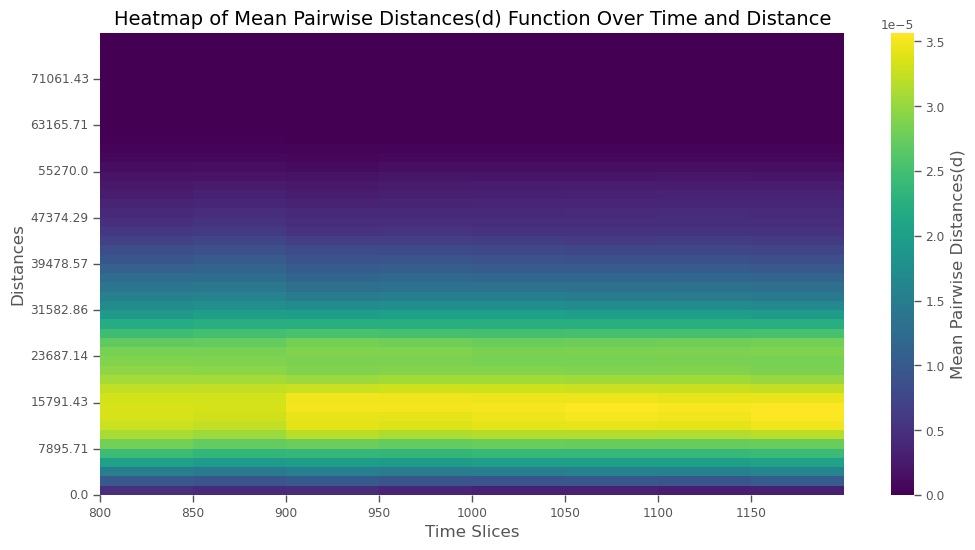
\includegraphics{analysis_files/figure-pdf/cell-10-output-2.png}

\paragraph{Complete Spatial
Randomness}\label{complete-spatial-randomness}

\paragraph{Figure S3: Heatmap of Pairwise Distance Density versus Time
for CSR based on Angkor's
Temples}\label{figure-s3-heatmap-of-pairwise-distance-density-versus-time-for-csr-based-on-angkors-temples}

\begin{Shaded}
\begin{Highlighting}[]
\CommentTok{\# Get MC iterations for incorporating chronological uncertainty and CSR}
\NormalTok{csr\_simulations\_angkor }\OperatorTok{=}\NormalTok{ clustering.mc\_samples(}
\NormalTok{    points, }
\NormalTok{    time\_slices }\OperatorTok{=}\NormalTok{ time\_slices,  }
\NormalTok{    num\_iterations }\OperatorTok{=}\NormalTok{ num\_iterations,}
\NormalTok{    null\_model}\OperatorTok{=}\NormalTok{clustering.csr\_sample,}
\NormalTok{    x\_min}\OperatorTok{=}\NormalTok{x\_min, }
\NormalTok{    x\_max}\OperatorTok{=}\NormalTok{x\_max,}
\NormalTok{    y\_min}\OperatorTok{=}\NormalTok{y\_min, }
\NormalTok{    y\_max}\OperatorTok{=}\NormalTok{y\_max}
\NormalTok{)}

\CommentTok{\# Calulate the pairwise distances for the CSR sample}
\NormalTok{csr\_pairwise\_density\_angkor, csr\_support\_angkor }\OperatorTok{=}\NormalTok{ clustering.temporal\_pairwise(}
\NormalTok{    csr\_simulations\_angkor, }
\NormalTok{    time\_slices, }
\NormalTok{    bw }\OperatorTok{=}\NormalTok{ pair\_bw, }
\NormalTok{    use\_kde }\OperatorTok{=}\NormalTok{ use\_kde,}
\NormalTok{    kde\_sample\_n}\OperatorTok{=}\NormalTok{kde\_sample\_n, }
\NormalTok{    max\_distance }\OperatorTok{=}\NormalTok{ max\_distance,}
\NormalTok{    kde\_custom}\OperatorTok{=}\NormalTok{kde\_custom}
\NormalTok{)}

\CommentTok{\# Visualize clustering with heatmap}
\NormalTok{clustering\_heatmap(}
\NormalTok{    csr\_pairwise\_density\_angkor,}
\NormalTok{    csr\_support\_angkor,}
\NormalTok{    time\_slices,}
\NormalTok{    result\_type}\OperatorTok{=}\StringTok{\textquotesingle{}Pairwise Distances\textquotesingle{}}
\NormalTok{)}
\end{Highlighting}
\end{Shaded}

\begin{verbatim}
(<Figure size 1200x600 with 2 Axes>,
 <Axes: title={'center': 'Heatmap of Mean Pairwise Distances(d) Function Over Time and Distance'}, xlabel='Time Slices', ylabel='Distances'>)
\end{verbatim}

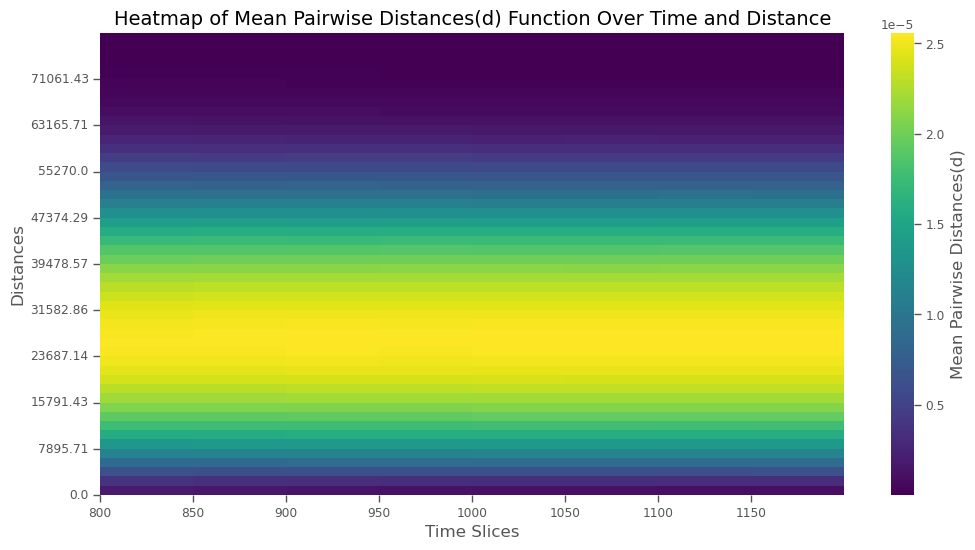
\includegraphics{analysis_files/figure-pdf/cell-11-output-2.png}

\paragraph{Figure S4: Heatmap of PDD Statistical Significance compared
to CSR for Angkor's
Temples}\label{figure-s4-heatmap-of-pdd-statistical-significance-compared-to-csr-for-angkors-temples}

\begin{Shaded}
\begin{Highlighting}[]
\CommentTok{\# Calculate the p{-}values for density differences between the observed points and }
\CommentTok{\# the simulated CSR baseline per distance and temporal slice}
\NormalTok{p\_diff\_array\_csr\_angkor, diff\_array\_csr\_angkor }\OperatorTok{=}\NormalTok{ clustering.p\_diff(}
\NormalTok{    pairwise\_density\_angkor, }
\NormalTok{    csr\_pairwise\_density\_angkor}
\NormalTok{)}

\CommentTok{\# Plot the heatmap of probabilities}
\NormalTok{pdiff\_heatmap(}
\NormalTok{    p\_diff\_array\_csr\_angkor,}
\NormalTok{    time\_slices,}
\NormalTok{    csr\_support\_angkor}
\NormalTok{)}
\end{Highlighting}
\end{Shaded}

\begin{verbatim}
(<Figure size 1200x600 with 2 Axes>,
 <Axes: title={'center': 'Probability Heat Map'}, xlabel='Time Slices', ylabel='Pairwise Distances'>)
\end{verbatim}

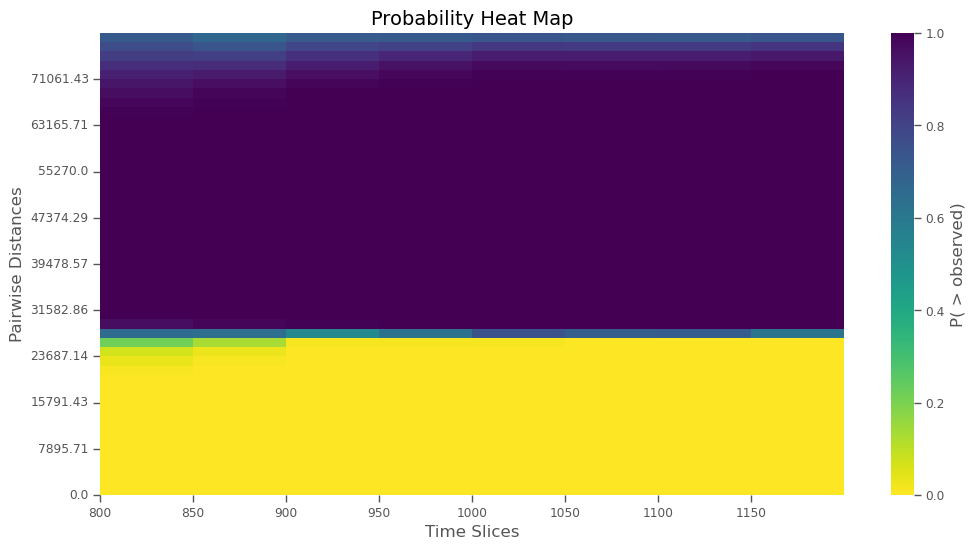
\includegraphics{analysis_files/figure-pdf/cell-12-output-2.png}

\paragraph{Baseline-Informed Spatial
Expectation}\label{baseline-informed-spatial-expectation}

\paragraph{Figure S5: Heatmap of PDD statistical significance compared
to BISE based on Angkor's
Temples}\label{figure-s5-heatmap-of-pdd-statistical-significance-compared-to-bise-based-on-angkors-temples}

\begin{Shaded}
\begin{Highlighting}[]
\CommentTok{\# Get MC iterations for incorporating chronological uncertainty with BISE}
\NormalTok{bise\_simulations\_angkor }\OperatorTok{=}\NormalTok{ clustering.mc\_samples(points, }
\NormalTok{                                         time\_slices, }
\NormalTok{                                         num\_iterations }\OperatorTok{=}\NormalTok{ num\_iterations,}
\NormalTok{                                         null\_model }\OperatorTok{=}\NormalTok{ clustering.bise)}

\CommentTok{\# Calulate the pairwise distances for the LISE sample}
\NormalTok{bise\_pairwise\_density\_angkor, bise\_support\_angkor }\OperatorTok{=}\NormalTok{ clustering.temporal\_pairwise(}
\NormalTok{    bise\_simulations\_angkor, }
\NormalTok{    time\_slices, }
\NormalTok{    bw }\OperatorTok{=}\NormalTok{ pair\_bw, }
\NormalTok{    use\_kde }\OperatorTok{=}\NormalTok{ use\_kde,}
\NormalTok{    kde\_sample\_n }\OperatorTok{=}\NormalTok{ kde\_sample\_n, }
\NormalTok{    max\_distance }\OperatorTok{=}\NormalTok{ max\_distance,}
\NormalTok{    kde\_custom }\OperatorTok{=}\NormalTok{ kde\_custom}
\NormalTok{)}

\CommentTok{\# Calculate the p{-}values for density differences between the observed points and }
\CommentTok{\# the simulated BISE baseline per distance and temporal slice}
\NormalTok{p\_diff\_array\_bise\_angkor, diff\_array\_bise\_angkor }\OperatorTok{=}\NormalTok{ clustering.p\_diff(}
\NormalTok{    pairwise\_density\_angkor, }
\NormalTok{    bise\_pairwise\_density\_angkor}
\NormalTok{)}
\end{Highlighting}
\end{Shaded}

\begin{Shaded}
\begin{Highlighting}[]
\CommentTok{\# Plot the heatmap of probabilities}
\NormalTok{fig, ax }\OperatorTok{=}\NormalTok{ pdiff\_heatmap(}
\NormalTok{    p\_diff\_array\_bise\_angkor,}
\NormalTok{    time\_slices,}
\NormalTok{    bise\_support\_angkor}
\NormalTok{)}

\CommentTok{\# Custom ticks and labels here}
\NormalTok{tick\_labels\_km }\OperatorTok{=}\NormalTok{ np.arange(}\DecValTok{0}\NormalTok{, bise\_support\_angkor.}\BuiltInTok{max}\NormalTok{() }\OperatorTok{/} \DecValTok{1000}\NormalTok{, }\DecValTok{10}\NormalTok{)}
\NormalTok{tick\_labels\_m }\OperatorTok{=}\NormalTok{ tick\_labels\_km }\OperatorTok{*} \DecValTok{1000}
\NormalTok{tick\_positions }\OperatorTok{=}\NormalTok{ np.interp(}
\NormalTok{    tick\_labels\_m, }
\NormalTok{    bise\_support\_angkor, }
\NormalTok{    np.arange(}\BuiltInTok{len}\NormalTok{(bise\_support\_angkor))}
\NormalTok{)}

\NormalTok{ax.set\_yticks(tick\_positions)}
\NormalTok{ax.set\_yticklabels(np.}\BuiltInTok{round}\NormalTok{(tick\_labels\_km, }\DecValTok{1}\NormalTok{))}
\NormalTok{ax.set\_ylabel(}\StringTok{"Distance (km)"}\NormalTok{)}

\NormalTok{ax.set\_xlabel(}\StringTok{"Time Slices (year CE)"}\NormalTok{)}
\NormalTok{ax.set\_title(}\StringTok{"P{-}Values for Angkor PDD (BISE null)"}\NormalTok{)}

\NormalTok{plt.savefig(}\StringTok{"../Output/dpdd\_hm\_angkor.svg"}\NormalTok{, bbox\_inches}\OperatorTok{=}\StringTok{\textquotesingle{}tight\textquotesingle{}}\NormalTok{)}
\NormalTok{plt.savefig(}\StringTok{"../Output/dpdd\_hm\_angkor.png"}\NormalTok{, bbox\_inches}\OperatorTok{=}\StringTok{\textquotesingle{}tight\textquotesingle{}}\NormalTok{)}
\end{Highlighting}
\end{Shaded}

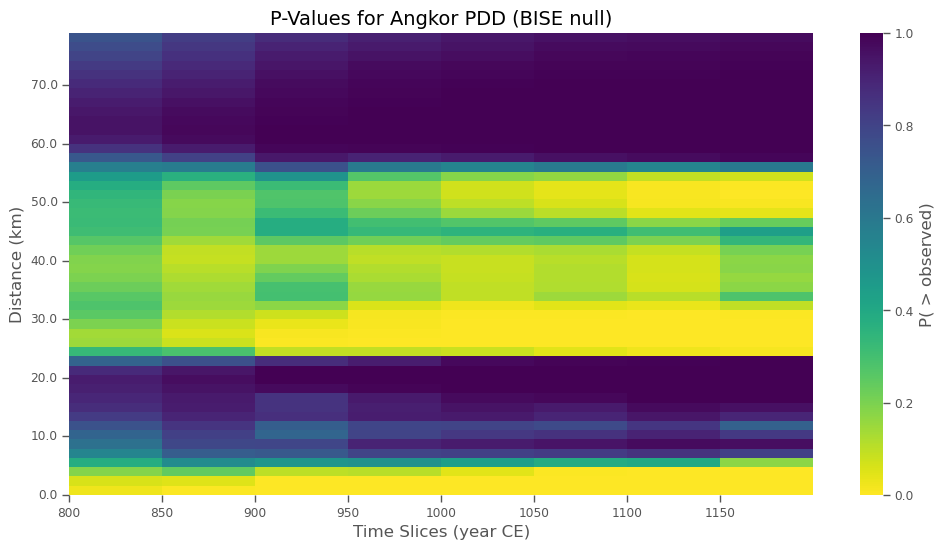
\includegraphics{analysis_files/figure-pdf/cell-14-output-1.png}

\paragraph{One Time Slice}\label{one-time-slice}

\paragraph{Figure S6: Time Slice of PDD for Angkor compared to Null
Models}\label{figure-s6-time-slice-of-pdd-for-angkor-compared-to-null-models}

\begin{Shaded}
\begin{Highlighting}[]
\ImportTok{from}\NormalTok{ chronocluster.utils }\ImportTok{import}\NormalTok{ plot\_pdd}

\NormalTok{time\_slice\_idx }\OperatorTok{=}\NormalTok{ np.where(time\_slices }\OperatorTok{==} \DecValTok{1000}\NormalTok{)[}\DecValTok{0}\NormalTok{][}\DecValTok{0}\NormalTok{]}

\CommentTok{\# List of density arrays}
\NormalTok{density\_arrays }\OperatorTok{=}\NormalTok{ [}
\NormalTok{    pairwise\_density\_angkor, }
\NormalTok{    csr\_pairwise\_density\_angkor, }
\NormalTok{    bise\_pairwise\_density\_angkor}
\NormalTok{]}

\CommentTok{\# Generate the plot and get the figure and axis objects}
\NormalTok{fig, ax }\OperatorTok{=}\NormalTok{ plot\_pdd(}
\NormalTok{    time\_slices}\OperatorTok{=}\NormalTok{time\_slices,}
\NormalTok{    time\_slice\_idx}\OperatorTok{=}\NormalTok{time\_slice\_idx,}
\NormalTok{    support}\OperatorTok{=}\NormalTok{support\_angkor,}
\NormalTok{    density\_arrays}\OperatorTok{=}\NormalTok{density\_arrays,}
\NormalTok{    quantiles}\OperatorTok{=}\NormalTok{[}\FloatTok{0.025}\NormalTok{, }\FloatTok{0.975}\NormalTok{],}
\NormalTok{    density\_names}\OperatorTok{=}\NormalTok{[}\StringTok{"Empirical"}\NormalTok{, }\StringTok{"CSR"}\NormalTok{, }\StringTok{"BISE"}\NormalTok{],}
\NormalTok{    colors}\OperatorTok{=}\NormalTok{[}\StringTok{"blue"}\NormalTok{, }\StringTok{"orange"}\NormalTok{, }\StringTok{"green"}\NormalTok{]}
\NormalTok{)}

\NormalTok{ax.set\_title(}\StringTok{"PDD Angkor 1000 CE"}\NormalTok{)}

\CommentTok{\# Get current tick positions and convert labels to km}
\NormalTok{x\_ticks }\OperatorTok{=}\NormalTok{ ax.get\_xticks()}
\NormalTok{ax.set\_xticklabels(np.}\BuiltInTok{round}\NormalTok{(x\_ticks }\OperatorTok{/} \DecValTok{1000}\NormalTok{, }\DecValTok{1}\NormalTok{))  }\CommentTok{\# e.g. 1000 → 1.0 km}

\CommentTok{\# Update axis label}
\NormalTok{ax.set\_xlabel(}\StringTok{"Distance (km)"}\NormalTok{)}

\CommentTok{\# Show the plot}
\NormalTok{plt.show()}

\NormalTok{fig.savefig(}\StringTok{"../Output/pdd\_null\_angkor.png"}\NormalTok{, dpi}\OperatorTok{=}\DecValTok{300}\NormalTok{, bbox\_inches}\OperatorTok{=}\StringTok{"tight"}\NormalTok{)}
\NormalTok{fig.savefig(}\StringTok{"../Output/pdd\_null\_angkor.svg"}\NormalTok{, bbox\_inches}\OperatorTok{=}\StringTok{"tight"}\NormalTok{)}
\end{Highlighting}
\end{Shaded}

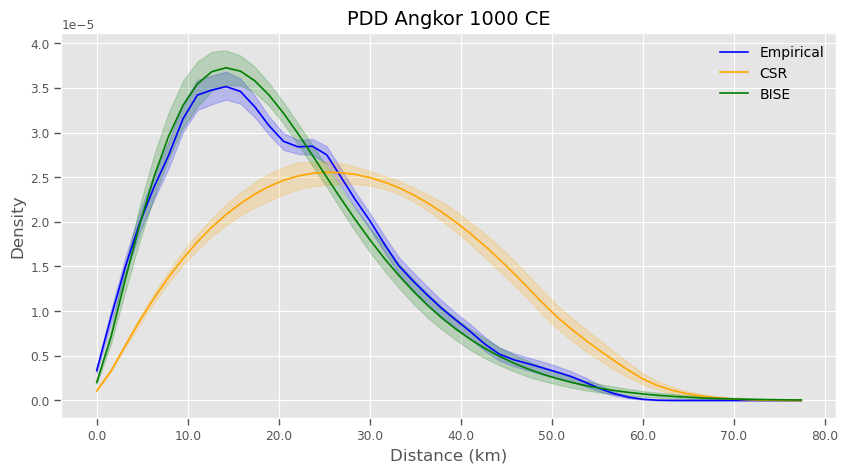
\includegraphics{analysis_files/figure-pdf/cell-15-output-1.png}

\paragraph{Figure S7: Difference between Angkor PDD and BISE Null at
1000
CE}\label{figure-s7-difference-between-angkor-pdd-and-bise-null-at-1000-ce}

\begin{Shaded}
\begin{Highlighting}[]
\CommentTok{\# List of density arrays}
\NormalTok{density\_arrays }\OperatorTok{=}\NormalTok{ [diff\_array\_bise\_angkor]}

\NormalTok{time\_slice\_idx }\OperatorTok{=}\NormalTok{ np.where(time\_slices }\OperatorTok{==} \DecValTok{1000}\NormalTok{)[}\DecValTok{0}\NormalTok{][}\DecValTok{0}\NormalTok{]}

\CommentTok{\# Generate the plot and get the figure and axis objects}
\NormalTok{fig1, ax1 }\OperatorTok{=}\NormalTok{ plot\_pdd(}
\NormalTok{    time\_slices}\OperatorTok{=}\NormalTok{time\_slices,}
\NormalTok{    time\_slice\_idx}\OperatorTok{=}\NormalTok{time\_slice\_idx,}
\NormalTok{    support}\OperatorTok{=}\NormalTok{support\_angkor,}
\NormalTok{    density\_arrays}\OperatorTok{=}\NormalTok{density\_arrays,}
\NormalTok{    quantiles}\OperatorTok{=}\NormalTok{[}\FloatTok{0.025}\NormalTok{, }\FloatTok{0.975}\NormalTok{],}
\NormalTok{    density\_names}\OperatorTok{=}\NormalTok{[}\StringTok{"Diff Array"}\NormalTok{],}
\NormalTok{    colors}\OperatorTok{=}\NormalTok{[}\StringTok{"blue"}\NormalTok{]}
\NormalTok{)}

\CommentTok{\# Add a horizontal line at y=0}
\NormalTok{ax1.axhline(y}\OperatorTok{=}\DecValTok{0}\NormalTok{, color}\OperatorTok{=}\StringTok{\textquotesingle{}red\textquotesingle{}}\NormalTok{, linestyle}\OperatorTok{=}\StringTok{\textquotesingle{}{-}{-}\textquotesingle{}}\NormalTok{, linewidth}\OperatorTok{=}\FloatTok{1.5}\NormalTok{)}

\NormalTok{ax1.set\_title(}\StringTok{"$\textbackslash{}Delta$PDD Angkor 1000 CE"}\NormalTok{)}
\CommentTok{\#ax1.set\_xlabel("Distance (m)")}

\CommentTok{\# Get current tick positions and convert labels to km}
\NormalTok{x\_ticks }\OperatorTok{=}\NormalTok{ ax1.get\_xticks()}
\NormalTok{ax1.set\_xticklabels(np.}\BuiltInTok{round}\NormalTok{(x\_ticks }\OperatorTok{/} \DecValTok{1000}\NormalTok{, }\DecValTok{1}\NormalTok{))  }\CommentTok{\# e.g. 1000 → 1.0 km}

\CommentTok{\# Update axis label}
\NormalTok{ax1.set\_xlabel(}\StringTok{"Distance (km)"}\NormalTok{)}

\CommentTok{\# Show the plot}
\NormalTok{plt.show()}

\NormalTok{fig.savefig(}\StringTok{"../Output/dpdd\_t1000\_angkor.png"}\NormalTok{, dpi}\OperatorTok{=}\DecValTok{300}\NormalTok{, bbox\_inches}\OperatorTok{=}\StringTok{"tight"}\NormalTok{)}
\NormalTok{fig.savefig(}\StringTok{"../Output/dpdd\_t1000\_angkor.svg"}\NormalTok{, bbox\_inches}\OperatorTok{=}\StringTok{"tight"}\NormalTok{)}
\end{Highlighting}
\end{Shaded}

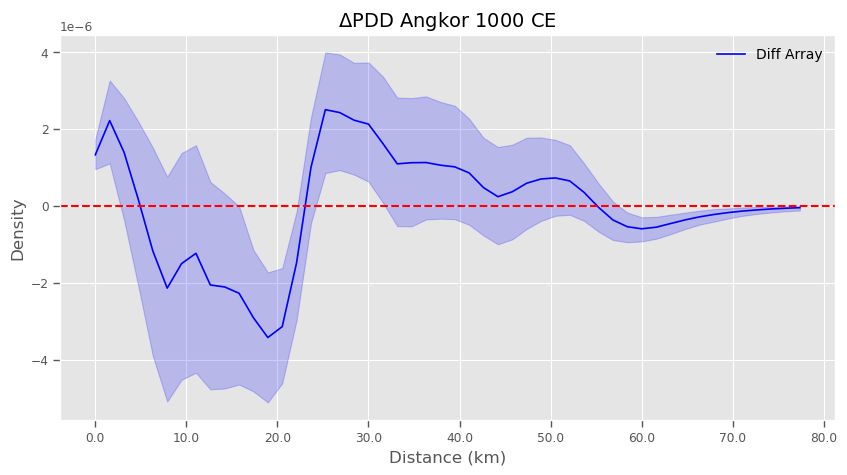
\includegraphics{analysis_files/figure-pdf/cell-16-output-1.png}

\paragraph{Series of Slices}\label{series-of-slices}

\paragraph{Figure S8: Difference between Angkor PDD and BISE Null at 4
Time
Slices}\label{figure-s8-difference-between-angkor-pdd-and-bise-null-at-4-time-slices}

\begin{Shaded}
\begin{Highlighting}[]
\CommentTok{\# List of time\_slice\_idx values}
\NormalTok{time\_slice\_indices }\OperatorTok{=}\NormalTok{ [}\DecValTok{0}\NormalTok{, }\DecValTok{2}\NormalTok{, }\DecValTok{4}\NormalTok{, }\DecValTok{6}\NormalTok{]}

\CommentTok{\# Create a figure and axes for subplots}
\CommentTok{\# Create a 2x2 grid of subplots}
\NormalTok{fig, axes }\OperatorTok{=}\NormalTok{ plt.subplots(}\DecValTok{2}\NormalTok{, }\DecValTok{2}\NormalTok{, figsize}\OperatorTok{=}\NormalTok{(}\DecValTok{10}\NormalTok{, }\DecValTok{10}\NormalTok{), sharey}\OperatorTok{=}\VariableTok{True}\NormalTok{)  }\CommentTok{\# 2 rows, 2 columns}

\NormalTok{axes\_flat }\OperatorTok{=}\NormalTok{ axes.flatten()}

\CommentTok{\# Loop through each time\_slice\_idx and generate the plots}
\ControlFlowTok{for}\NormalTok{ idx, (ax, time\_slice\_idx) }\KeywordTok{in} \BuiltInTok{enumerate}\NormalTok{(}\BuiltInTok{zip}\NormalTok{(axes\_flat, time\_slice\_indices)):}
    \CommentTok{\# Generate the plot for the current time\_slice\_idx}
\NormalTok{    fig, \_ }\OperatorTok{=}\NormalTok{ plot\_pdd(}
\NormalTok{        time\_slices}\OperatorTok{=}\NormalTok{time\_slices,}
\NormalTok{        time\_slice\_idx}\OperatorTok{=}\NormalTok{time\_slice\_idx,}
\NormalTok{        support}\OperatorTok{=}\NormalTok{support\_angkor,}
\NormalTok{        density\_arrays}\OperatorTok{=}\NormalTok{density\_arrays,}
\NormalTok{        quantiles}\OperatorTok{=}\NormalTok{[}\FloatTok{0.025}\NormalTok{, }\FloatTok{0.975}\NormalTok{],}
\NormalTok{        density\_names}\OperatorTok{=}\NormalTok{[}\StringTok{"$\textbackslash{}Delta$PDD"}\NormalTok{],}
\NormalTok{        colors}\OperatorTok{=}\NormalTok{[}\StringTok{"blue"}\NormalTok{],}
\NormalTok{        ax}\OperatorTok{=}\NormalTok{ax}
\NormalTok{    )}
    
    \CommentTok{\# Add a horizontal line (optional)}
\NormalTok{    ax.axhline(y}\OperatorTok{=}\DecValTok{0}\NormalTok{, color}\OperatorTok{=}\StringTok{\textquotesingle{}red\textquotesingle{}}\NormalTok{, linestyle}\OperatorTok{=}\StringTok{\textquotesingle{}{-}{-}\textquotesingle{}}\NormalTok{, linewidth}\OperatorTok{=}\FloatTok{1.5}\NormalTok{)}
    
    \CommentTok{\# Add a title for each panel}
\NormalTok{    ax.set\_title(}\SpecialStringTok{f"Time Slice: }\SpecialCharTok{\{}\NormalTok{time\_slices[time\_slice\_idx]}\SpecialCharTok{\}}\SpecialStringTok{"}\NormalTok{)}
\NormalTok{    ax.set\_xlabel(}\StringTok{"Distance (m)"}\NormalTok{)}
    \CommentTok{\# Get current tick positions and convert labels to km}
\NormalTok{    x\_ticks }\OperatorTok{=}\NormalTok{ ax.get\_xticks()}
\NormalTok{    ax.set\_xticklabels(np.}\BuiltInTok{round}\NormalTok{(x\_ticks }\OperatorTok{/} \DecValTok{1000}\NormalTok{, }\DecValTok{1}\NormalTok{))  }\CommentTok{\# e.g. 1000 → 1.0 km}

    \CommentTok{\# Update axis label}
\NormalTok{    ax.set\_xlabel(}\StringTok{"Distance (km)"}\NormalTok{)}

\CommentTok{\# Adjust layout and show the stitched plot}
\NormalTok{plt.tight\_layout(rect}\OperatorTok{=}\NormalTok{[}\DecValTok{0}\NormalTok{, }\DecValTok{0}\NormalTok{, }\DecValTok{1}\NormalTok{, }\FloatTok{0.95}\NormalTok{])}
\NormalTok{fig.suptitle(}\StringTok{"$\textbackslash{}Delta$PDD Series for Angkor"}\NormalTok{)}
\NormalTok{plt.show()}

\NormalTok{fig.savefig(}\StringTok{"../Output/dpdd\_series\_angkor.png"}\NormalTok{, dpi}\OperatorTok{=}\DecValTok{300}\NormalTok{, bbox\_inches}\OperatorTok{=}\StringTok{"tight"}\NormalTok{)}
\NormalTok{fig.savefig(}\StringTok{"../Output/dpdd\_series\_angkor.svg"}\NormalTok{, bbox\_inches}\OperatorTok{=}\StringTok{"tight"}\NormalTok{)}
\end{Highlighting}
\end{Shaded}

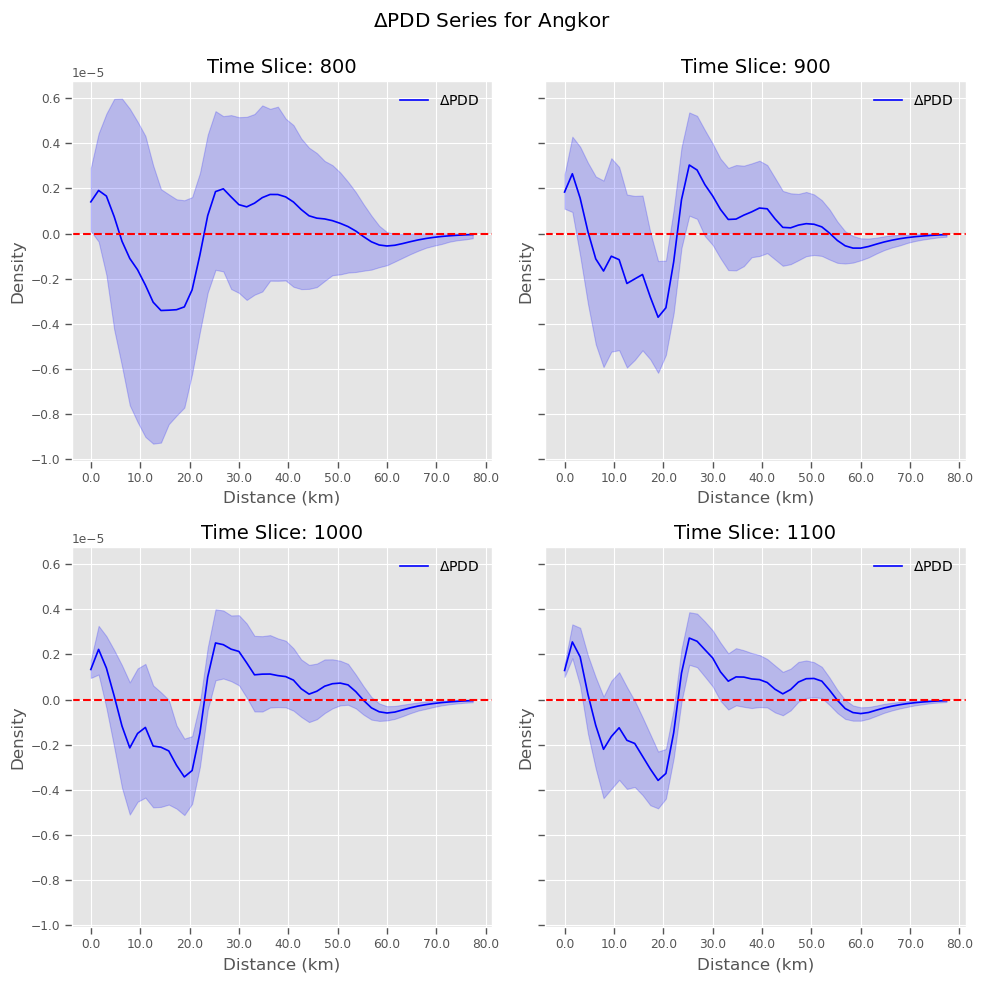
\includegraphics{analysis_files/figure-pdf/cell-17-output-1.png}

\subsection{Hampshire County at
Doomsday}\label{hampshire-county-at-doomsday}

\subsubsection{Data Wrangling}\label{data-wrangling-1}

\begin{Shaded}
\begin{Highlighting}[]
\CommentTok{\# data wrangling}
\NormalTok{doomsday\_places }\OperatorTok{=}\NormalTok{ pd.read\_csv(}\StringTok{\textquotesingle{}../Data/doomsday\_places.csv\textquotesingle{}}\NormalTok{)}
\NormalTok{doomsday\_places }\OperatorTok{=}\NormalTok{ doomsday\_places.dropna(subset}\OperatorTok{=}\NormalTok{[}\StringTok{\textquotesingle{}easting\textquotesingle{}}\NormalTok{, }\StringTok{\textquotesingle{}northing\textquotesingle{}}\NormalTok{])}
\NormalTok{doomsday\_places}
\end{Highlighting}
\end{Shaded}

\begin{longtable}[]{@{}llllllllllllllll@{}}
\toprule\noalign{}
& PlacesIdx & County & Phillimore & Hundred & Vill & Area & XRefs &
OSrefs & OScodes & lat & lon & easting & northing & start\_date &
end\_date \\
\midrule\noalign{}
\endhead
\bottomrule\noalign{}
\endlastfoot
0 & 1 & WOR & 15,8 & `Doddingtree\textquotesingle{} & Abberley & NaN &
NaN & SO7567 & NaN & 52.300561 & -2.368032 & 375000.0 & 267000.0 & 1066
& 1086 \\
1 & 6 & ESS & 20,20. 24,51. 34,16 & `Winstree\textquotesingle{} &
Abberton & NaN & NaN & TL9919 & NaN & 51.834157 & 0.886905 & 599000.0 &
219000.0 & 1066 & 1086 \\
2 & 11 & WOR & 9,1a & Pershore & Abberton & NaN & NaN & SO9953 & NaN &
52.175269 & -2.016034 & 399000.0 & 253000.0 & 1066 & 1086 \\
3 & 16 & DOR & 13,1 & `Uggescombe\textquotesingle{} & Abbotsbury & NaN &
NaN & SY5785 & NaN & 50.663064 & -2.609752 & 357000.0 & 85000.0 & 1066 &
1086 \\
4 & 21 & DEV & 5,6 & Merton & Abbotsham & NaN & NaN & SS4226 & NaN &
51.011615 & -4.253705 & 242000.0 & 126000.0 & 1066 & 1086 \\
... & ... & ... & ... & ... & ... & ... & ... & ... & ... & ... & ... &
... & ... & ... & ... \\
13453 & 73861 & STS & 2,22 & Offlow & Yoxall & NaN & NaN & SK1419 & NaN
& 52.768434 & -1.793938 & 414000.0 & 319000.0 & 1066 & 1086 \\
13454 & 73866 & SUF & 7,18. 44,4 & `Blything\textquotesingle{} & Yoxford
& NaN & NaN & TM3968 & NaN & 52.258228 & 1.500634 & 639000.0 & 268000.0
& 1066 & 1086 \\
13455 & 73871 & CHS & FT1,4 & Ati\textquotesingle s Cross & Ysceifiog &
Ati\textquotesingle s Cross & NaN & SJ1571 & NaN & 53.229229 & -3.274776
& 315000.0 & 371000.0 & 1066 & 1086 \\
13456 & 73876 & DEV & 6,3 & North Tawton & Zeal Monachorum & NaN & NaN &
SS7103 & NaN & 50.812135 & -3.832415 & 271000.0 & 103000.0 & 1066 &
1086 \\
13457 & 73881 & WIL & 64,1. 67,32 & Mere & Zeals & NaN & NaN & ST7831 &
NaN & 51.077890 & -2.315416 & 378000.0 & 131000.0 & 1066 & 1086 \\
\end{longtable}

Includes removing two problematic points in the data with a likely
incorrect county labels.

\begin{Shaded}
\begin{Highlighting}[]
\CommentTok{\# isolating Hampshire for comparison with Angkor}
\NormalTok{counties }\OperatorTok{=}\NormalTok{ [}\StringTok{\textquotesingle{}HAM\textquotesingle{}}\NormalTok{]}
\NormalTok{doomsday\_df }\OperatorTok{=}\NormalTok{ doomsday\_places[doomsday\_places[}\StringTok{\textquotesingle{}County\textquotesingle{}}\NormalTok{].isin(counties)]}

\CommentTok{\# I know there is a probable county designation error for the following point }
\CommentTok{\# (observed in QGIS as an kind of spatial outlier surrounded by points  with a }
\CommentTok{\# different designation and appears to be a duplicate point where the alternate }
\CommentTok{\# one has the same county designation as the other surrounding points)}

\CommentTok{\# PlacesIdx of the mislabelled point is 10221 while the alternate is 10226}
\NormalTok{drop\_idx }\OperatorTok{=}\NormalTok{ doomsday\_df[doomsday\_df[}\StringTok{\textquotesingle{}PlacesIdx\textquotesingle{}}\NormalTok{].isin([}\DecValTok{10221}\NormalTok{, }\DecValTok{30086}\NormalTok{])].index}
\NormalTok{doomsday\_df }\OperatorTok{=}\NormalTok{ doomsday\_df.drop(drop\_idx)}
\end{Highlighting}
\end{Shaded}

\subsubsection{Create Points List}\label{create-points-list-1}

\begin{Shaded}
\begin{Highlighting}[]
\NormalTok{doomsday\_points }\OperatorTok{=}\NormalTok{ [}
\NormalTok{    clustering.Point(}
\NormalTok{        x}\OperatorTok{=}\NormalTok{row[}\StringTok{\textquotesingle{}easting\textquotesingle{}}\NormalTok{],}
\NormalTok{        y}\OperatorTok{=}\NormalTok{row[}\StringTok{\textquotesingle{}northing\textquotesingle{}}\NormalTok{],}
\NormalTok{        start\_distribution }\OperatorTok{=}\NormalTok{ ddelta(}\DecValTok{1066}\NormalTok{),}
\NormalTok{        end\_distribution }\OperatorTok{=}\NormalTok{ ddelta(}\DecValTok{1086}\NormalTok{)}
\NormalTok{    )}
    \ControlFlowTok{for}\NormalTok{ \_, row }\KeywordTok{in}\NormalTok{ doomsday\_df.iterrows()}
\NormalTok{]}

\CommentTok{\# just double check the first ten look right}
\NormalTok{doomsday\_points[:}\DecValTok{10}\NormalTok{]}
\end{Highlighting}
\end{Shaded}

\begin{verbatim}
[Point(x=456000.0, y=134000.0, start_distribution=ddelta(d=1066), end_distribution=ddelta(d=1086)),
 Point(x=458000.0, y=88000.0, start_distribution=ddelta(d=1066), end_distribution=ddelta(d=1086)),
 Point(x=459000.0, y=86000.0, start_distribution=ddelta(d=1066), end_distribution=ddelta(d=1086)),
 Point(x=435000.0, y=86000.0, start_distribution=ddelta(d=1066), end_distribution=ddelta(d=1086)),
 Point(x=456000.0, y=83000.0, start_distribution=ddelta(d=1066), end_distribution=ddelta(d=1086)),
 Point(x=447000.0, y=117000.0, start_distribution=ddelta(d=1066), end_distribution=ddelta(d=1086)),
 Point(x=427000.0, y=107000.0, start_distribution=ddelta(d=1066), end_distribution=ddelta(d=1086)),
 Point(x=458000.0, y=133000.0, start_distribution=ddelta(d=1066), end_distribution=ddelta(d=1086)),
 Point(x=471000.0, y=139000.0, start_distribution=ddelta(d=1066), end_distribution=ddelta(d=1086)),
 Point(x=460000.0, y=98000.0, start_distribution=ddelta(d=1066), end_distribution=ddelta(d=1086))]
\end{verbatim}

\subsubsection{Define Time Slices and Spatial
Limits}\label{define-time-slices-and-spatial-limits}

\begin{Shaded}
\begin{Highlighting}[]
\CommentTok{\# Define the time slices}
\NormalTok{start\_time }\OperatorTok{=} \DecValTok{1066}
\NormalTok{end\_time }\OperatorTok{=} \DecValTok{1086}
\NormalTok{time\_interval }\OperatorTok{=} \DecValTok{5}
\NormalTok{time\_slices\_ham }\OperatorTok{=}\NormalTok{ np.arange(start\_time, end\_time, time\_interval)}

\CommentTok{\# Get a bounding box for use later and to extract sensible distance limits}
\NormalTok{x\_min, y\_min, x\_max, y\_max }\OperatorTok{=}\NormalTok{ get\_box(doomsday\_points)}
\NormalTok{max\_distance }\OperatorTok{=}\NormalTok{ np.ceil(np.sqrt((x\_max }\OperatorTok{{-}}\NormalTok{ x\_min)}\OperatorTok{**}\DecValTok{2} \OperatorTok{+}\NormalTok{ (y\_max }\OperatorTok{{-}}\NormalTok{ y\_min)}\OperatorTok{**}\DecValTok{2}\NormalTok{))}
\end{Highlighting}
\end{Shaded}

\paragraph{Figure S9: Spacetime Volume of Hampshire's
Estates}\label{figure-s9-spacetime-volume-of-hampshires-estates}

\begin{Shaded}
\begin{Highlighting}[]
\CommentTok{\# Custom styling parameters}
\NormalTok{style\_params }\OperatorTok{=}\NormalTok{ \{}
    \StringTok{\textquotesingle{}start\_mean\_color\textquotesingle{}}\NormalTok{: }\VariableTok{None}\NormalTok{,  }\CommentTok{\# Do not plot start mean points}
    \StringTok{\textquotesingle{}end\_mean\_color\textquotesingle{}}\NormalTok{: }\VariableTok{None}\NormalTok{, }\CommentTok{\# Do not plot end mean points}
    \StringTok{\textquotesingle{}mean\_point\_size\textquotesingle{}}\NormalTok{: }\DecValTok{10}\NormalTok{,}
    \StringTok{\textquotesingle{}cylinder\_color\textquotesingle{}}\NormalTok{: (}\FloatTok{0.3}\NormalTok{, }\FloatTok{0.3}\NormalTok{, }\FloatTok{0.3}\NormalTok{),  }\CommentTok{\# Dark grey}
    \StringTok{\textquotesingle{}ppf\_limits\textquotesingle{}}\NormalTok{: (}\FloatTok{0.05}\NormalTok{, }\FloatTok{0.95}\NormalTok{),  }\CommentTok{\# Use different ppf limits}
    \StringTok{\textquotesingle{}shadow\_color\textquotesingle{}}\NormalTok{: (}\FloatTok{0.4}\NormalTok{, }\FloatTok{0.4}\NormalTok{, }\FloatTok{0.4}\NormalTok{),  }\CommentTok{\# grey}
    \StringTok{\textquotesingle{}shadow\_size\textquotesingle{}}\NormalTok{: }\DecValTok{10}\NormalTok{,}
    \StringTok{\textquotesingle{}time\_slice\_color\textquotesingle{}}\NormalTok{: (}\FloatTok{0.5}\NormalTok{, }\FloatTok{0.5}\NormalTok{, }\FloatTok{0.5}\NormalTok{),  }\CommentTok{\# Grey}
    \StringTok{\textquotesingle{}time\_slice\_alpha\textquotesingle{}}\NormalTok{: }\FloatTok{0.3}\NormalTok{,}
    \StringTok{\textquotesingle{}time\_slice\_point\_color\textquotesingle{}}\NormalTok{: (}\DecValTok{0}\NormalTok{, }\DecValTok{0}\NormalTok{, }\DecValTok{0}\NormalTok{),  }\CommentTok{\# Black}
\NormalTok{\}}

\CommentTok{\# Plot the points using the chrono\_plot function with }
\CommentTok{\# custom styling and a time slice plane}
\NormalTok{ax\_stv\_doomsday, fig\_stv\_doomsday }\OperatorTok{=}\NormalTok{ chrono\_plot(}
\NormalTok{    doomsday\_points, }
\NormalTok{    style\_params}\OperatorTok{=}\NormalTok{style\_params, }
\NormalTok{    time\_slice}\OperatorTok{=}\DecValTok{1076}\NormalTok{,}
\NormalTok{    title}\OperatorTok{=}\StringTok{\textquotesingle{}Hamphsire\textquotesingle{}}
\NormalTok{)}
\NormalTok{ax\_stv\_doomsday.set\_box\_aspect(}\VariableTok{None}\NormalTok{, zoom}\OperatorTok{=}\FloatTok{0.85}\NormalTok{)}
\NormalTok{plt.savefig(}\StringTok{"../Output/spacetime\_volume\_Hampshire.svg"}\NormalTok{, bbox\_inches}\OperatorTok{=}\StringTok{\textquotesingle{}tight\textquotesingle{}}\NormalTok{)}
\end{Highlighting}
\end{Shaded}

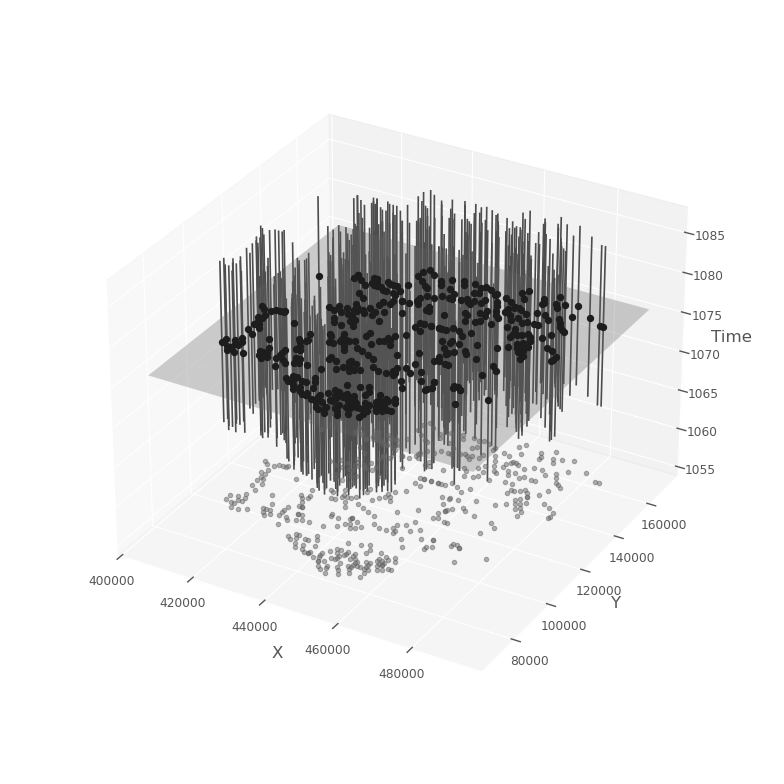
\includegraphics{analysis_files/figure-pdf/cell-22-output-1.png}

Figure S10: 2D Spatiotemporal Point Scatters of Angkor's Temples and
Hampshire's Estates

\begin{Shaded}
\begin{Highlighting}[]
\CommentTok{\# Style}
\NormalTok{scatter\_style }\OperatorTok{=}\NormalTok{ \{}
    \StringTok{"point\_color"}\NormalTok{: (}\DecValTok{0}\NormalTok{, }\DecValTok{0}\NormalTok{, }\DecValTok{0}\NormalTok{),}
    \StringTok{"point\_size"}\NormalTok{: }\DecValTok{10}\NormalTok{,}
\NormalTok{\}}

\NormalTok{width\_mm }\OperatorTok{=} \DecValTok{90}  \CommentTok{\# Example width in mm}
\NormalTok{width\_inch }\OperatorTok{=}\NormalTok{ width\_mm }\OperatorTok{/} \FloatTok{25.4}  \CommentTok{\# Convert mm to inches}

\CommentTok{\# Create a figure with two subplots side by side (1 row, 2 columns)}
\NormalTok{fig, (ax\_2d\_angkor, ax\_2d\_hampshire) }\OperatorTok{=}\NormalTok{ plt.subplots(}
    \DecValTok{1}\NormalTok{, }
    \DecValTok{2}\NormalTok{, }
\NormalTok{    figsize }\OperatorTok{=}\NormalTok{ (}\DecValTok{2} \OperatorTok{*}\NormalTok{ width\_inch, }\FloatTok{1.15} \OperatorTok{*}\NormalTok{ width\_inch)}
\NormalTok{)}

\NormalTok{y\_delta }\OperatorTok{=} \FloatTok{0.18e6}

\CommentTok{\# Plot for Angkor}
\NormalTok{ax\_2d\_angkor, fig\_2d\_angkor }\OperatorTok{=}\NormalTok{ chrono\_plot2d(}
\NormalTok{    angkor\_points,}
\NormalTok{    time }\OperatorTok{=} \DecValTok{1000}\NormalTok{,}
\NormalTok{    style\_params }\OperatorTok{=}\NormalTok{ scatter\_style,}
\NormalTok{    crs }\OperatorTok{=} \StringTok{"EPSG:32648"}\NormalTok{,}
\NormalTok{    basemap\_provider }\OperatorTok{=}\NormalTok{ ctx.providers.CartoDB.Voyager,}
\NormalTok{    ax }\OperatorTok{=}\NormalTok{ ax\_2d\_angkor,}
\NormalTok{)}

\NormalTok{ax\_2d\_angkor.set\_title(}\StringTok{"Angkor 1000 CE"}\NormalTok{, fontsize }\OperatorTok{=} \DecValTok{10}\NormalTok{)}
\NormalTok{ax\_2d\_angkor.set\_xlabel(}\StringTok{"Easting"}\NormalTok{, fontsize }\OperatorTok{=} \DecValTok{8}\NormalTok{)}
\NormalTok{ax\_2d\_angkor.set\_ylabel(}\StringTok{"Northing"}\NormalTok{, fontsize }\OperatorTok{=} \DecValTok{8}\NormalTok{)}
\NormalTok{ax\_2d\_angkor.tick\_params(axis }\OperatorTok{=} \StringTok{\textquotesingle{}both\textquotesingle{}}\NormalTok{, labelsize }\OperatorTok{=} \DecValTok{8}\NormalTok{)}

\CommentTok{\# Plot for Hampshire}
\NormalTok{ax\_2d\_hampshire, fig\_2d\_hampshire }\OperatorTok{=}\NormalTok{ chrono\_plot2d(}
\NormalTok{    doomsday\_points,}
\NormalTok{    time }\OperatorTok{=} \DecValTok{1076}\NormalTok{,}
\NormalTok{    style\_params }\OperatorTok{=}\NormalTok{ scatter\_style,}
\NormalTok{    crs }\OperatorTok{=} \StringTok{"EPSG:27700"}\NormalTok{,}
\NormalTok{    basemap\_provider }\OperatorTok{=}\NormalTok{ ctx.providers.CartoDB.Voyager,}
\NormalTok{    ax }\OperatorTok{=}\NormalTok{ ax\_2d\_hampshire,}
\NormalTok{)}

\NormalTok{ax\_2d\_hampshire.ticklabel\_format(style }\OperatorTok{=} \StringTok{\textquotesingle{}sci\textquotesingle{}}\NormalTok{, scilimits }\OperatorTok{=}\NormalTok{ (}\DecValTok{0}\NormalTok{, }\DecValTok{0}\NormalTok{))}
\NormalTok{ax\_2d\_hampshire.set\_title(}\StringTok{"Hampshire 1076 CE"}\NormalTok{, fontsize }\OperatorTok{=} \DecValTok{10}\NormalTok{)}
\NormalTok{ax\_2d\_hampshire.set\_xlabel(}\StringTok{"Easting"}\NormalTok{, fontsize }\OperatorTok{=} \DecValTok{8}\NormalTok{)}
\NormalTok{ax\_2d\_hampshire.set\_ylabel(}\StringTok{"Northing"}\NormalTok{, fontsize }\OperatorTok{=} \DecValTok{8}\NormalTok{)}
\NormalTok{ax\_2d\_hampshire.tick\_params(axis }\OperatorTok{=} \StringTok{\textquotesingle{}both\textquotesingle{}}\NormalTok{, labelsize }\OperatorTok{=} \DecValTok{8}\NormalTok{)}

\NormalTok{inclusion\_legend(}
\NormalTok{    ax }\OperatorTok{=} \VariableTok{None}\NormalTok{, }
\NormalTok{    shared }\OperatorTok{=} \VariableTok{True}\NormalTok{, }
\NormalTok{    fig }\OperatorTok{=}\NormalTok{ fig, }
\NormalTok{    alphas }\OperatorTok{=}\NormalTok{ [}\FloatTok{0.2}\NormalTok{, }\FloatTok{0.5}\NormalTok{, }\FloatTok{0.8}\NormalTok{, }\FloatTok{1.0}\NormalTok{]}
\NormalTok{)}

\CommentTok{\# Adjust layout}
\NormalTok{fig.tight\_layout(rect }\OperatorTok{=}\NormalTok{ [}\DecValTok{0}\NormalTok{, }\DecValTok{1}\NormalTok{, }\DecValTok{0}\NormalTok{, }\DecValTok{1}\NormalTok{])}

\CommentTok{\# Save figure}
\NormalTok{plt.savefig(}
    \StringTok{"../Output/combined\_inclusion\_scatter.svg"}\NormalTok{, }
\NormalTok{    bbox\_inches }\OperatorTok{=} \StringTok{"tight"}\NormalTok{, }
\NormalTok{    dpi }\OperatorTok{=} \DecValTok{300}
\NormalTok{)}
\NormalTok{plt.savefig(}
    \StringTok{"../Output/combined\_inclusion\_scatter.png"}\NormalTok{, }
\NormalTok{    bbox\_inches }\OperatorTok{=} \StringTok{"tight"}\NormalTok{, }
\NormalTok{    dpi }\OperatorTok{=} \DecValTok{300}\NormalTok{)}
\end{Highlighting}
\end{Shaded}

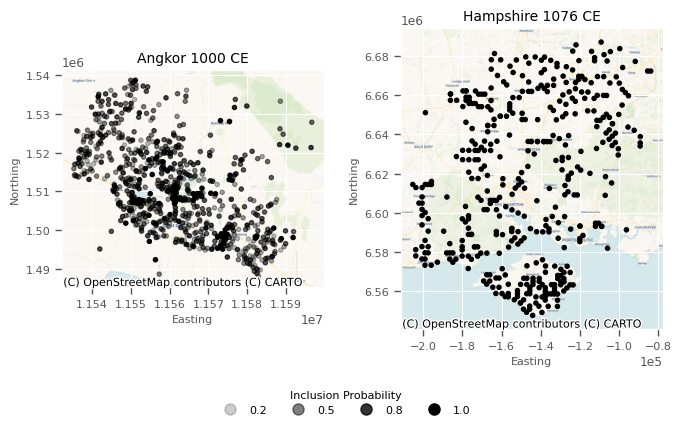
\includegraphics{analysis_files/figure-pdf/cell-23-output-1.png}

\paragraph{Figure S11: Spacetime Volumes for Angkor and Hampshire
Combined}\label{figure-s11-spacetime-volumes-for-angkor-and-hampshire-combined}

\begin{Shaded}
\begin{Highlighting}[]
\NormalTok{fig, axs }\OperatorTok{=}\NormalTok{ plt.subplots(}
    \DecValTok{1}\NormalTok{, }
    \DecValTok{2}\NormalTok{, }
\NormalTok{    figsize }\OperatorTok{=}\NormalTok{ (}\DecValTok{16}\NormalTok{, }\DecValTok{6}\NormalTok{), }
\NormalTok{    subplot\_kw }\OperatorTok{=}\NormalTok{ \{}\StringTok{"projection"}\NormalTok{: }\StringTok{"3d"}\NormalTok{\}}
\NormalTok{)}

\CommentTok{\# Plot both datasets into subplots}
\NormalTok{chrono\_plot(}
\NormalTok{    points, }
\NormalTok{    ax }\OperatorTok{=}\NormalTok{ axs[}\DecValTok{0}\NormalTok{], }
\NormalTok{    style\_params }\OperatorTok{=}\NormalTok{ style\_params, }
\NormalTok{    time\_slice }\OperatorTok{=} \DecValTok{1000}
\NormalTok{)}
\NormalTok{chrono\_plot(}
\NormalTok{    doomsday\_points, }
\NormalTok{    ax }\OperatorTok{=}\NormalTok{ axs[}\DecValTok{1}\NormalTok{], }
\NormalTok{    style\_params }\OperatorTok{=}\NormalTok{ style\_params, }
\NormalTok{    time\_slice }\OperatorTok{=} \DecValTok{1068}
\NormalTok{)}

\CommentTok{\# Add panel labels}
\NormalTok{fig.text(}
    \FloatTok{0.05}\NormalTok{, }
    \FloatTok{0.95}\NormalTok{, }
    \StringTok{"Angkor"}\NormalTok{, }
\NormalTok{    fontsize }\OperatorTok{=} \DecValTok{16}\NormalTok{, }
\NormalTok{    weight }\OperatorTok{=} \StringTok{"bold"}\NormalTok{, }
\NormalTok{    transform }\OperatorTok{=}\NormalTok{ fig.transFigure}
\NormalTok{)}
\NormalTok{fig.text(}
    \FloatTok{0.52}\NormalTok{, }
    \FloatTok{0.95}\NormalTok{, }
    \StringTok{"Hampshire"}\NormalTok{, }
\NormalTok{    fontsize }\OperatorTok{=} \DecValTok{16}\NormalTok{, }
\NormalTok{    weight }\OperatorTok{=} \StringTok{"bold"}\NormalTok{, }
\NormalTok{    transform }\OperatorTok{=}\NormalTok{ fig.transFigure}
\NormalTok{)}

\CommentTok{\# Save combined figure}
\NormalTok{fig.tight\_layout()}

\CommentTok{\# Z{-}axis labels (use labelpad to bring them in from the edge)}
\NormalTok{axs[}\DecValTok{0}\NormalTok{].set\_zlabel(}\StringTok{"Time"}\NormalTok{, labelpad }\OperatorTok{=} \DecValTok{10}\NormalTok{)}
\NormalTok{axs[}\DecValTok{0}\NormalTok{].ticklabel\_format(style }\OperatorTok{=} \StringTok{\textquotesingle{}plain\textquotesingle{}}\NormalTok{, axis }\OperatorTok{=} \StringTok{\textquotesingle{}both\textquotesingle{}}\NormalTok{)  }\CommentTok{\# or \textquotesingle{}y\textquotesingle{} or \textquotesingle{}both\textquotesingle{}}
\NormalTok{axs[}\DecValTok{1}\NormalTok{].set\_zlabel(}\StringTok{"Time"}\NormalTok{, labelpad }\OperatorTok{=} \DecValTok{10}\NormalTok{)}
\NormalTok{axs[}\DecValTok{1}\NormalTok{].ticklabel\_format(style }\OperatorTok{=} \StringTok{\textquotesingle{}plain\textquotesingle{}}\NormalTok{, axis }\OperatorTok{=} \StringTok{\textquotesingle{}both\textquotesingle{}}\NormalTok{)  }\CommentTok{\# or \textquotesingle{}y\textquotesingle{} or \textquotesingle{}both\textquotesingle{}}


\NormalTok{fig.savefig(}
    \StringTok{"../Output/spacetime\_volume\_combined.png"}\NormalTok{, }
\NormalTok{    dpi }\OperatorTok{=} \DecValTok{300}\NormalTok{, }
\NormalTok{    bbox\_inches }\OperatorTok{=} \StringTok{"tight"}\NormalTok{, }
\NormalTok{    pad\_inches }\OperatorTok{=} \FloatTok{1.0}
\NormalTok{)}
\NormalTok{fig.savefig(}
    \StringTok{"../Output/spacetime\_volume\_combined.svg"}\NormalTok{, }
\NormalTok{    bbox\_inches }\OperatorTok{=} \StringTok{"tight"}\NormalTok{, }
\NormalTok{    pad\_inches }\OperatorTok{=} \FloatTok{1.0}
\NormalTok{)}
\end{Highlighting}
\end{Shaded}

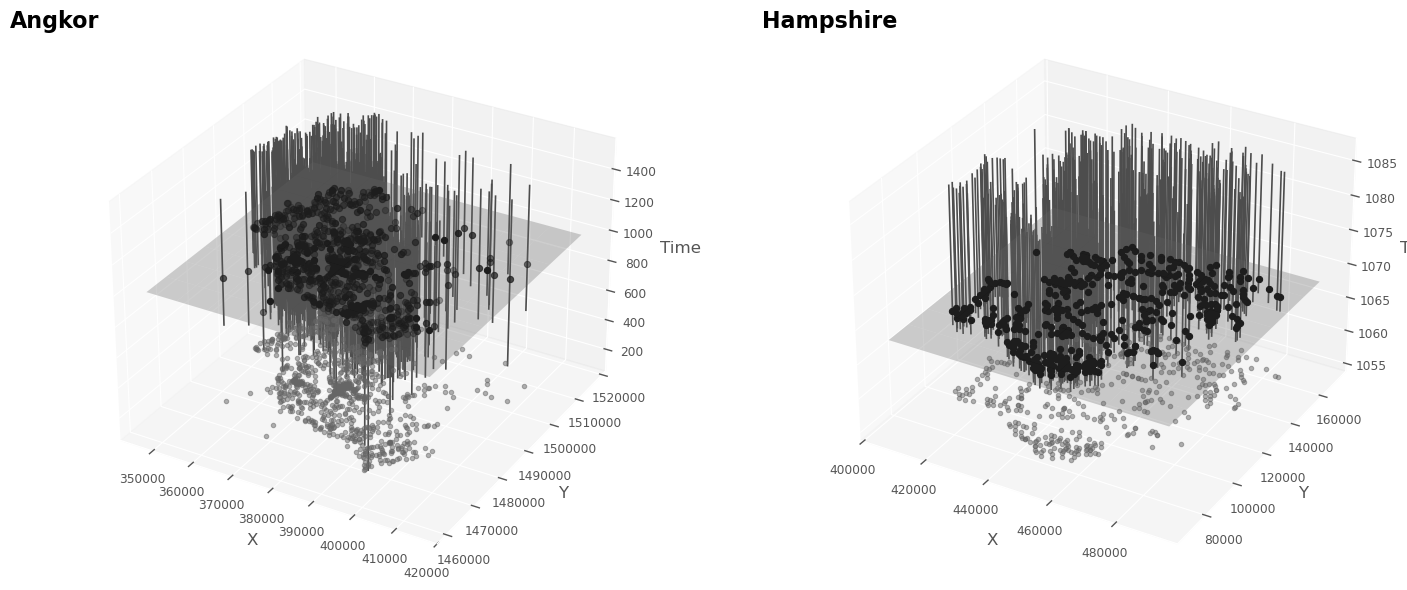
\includegraphics{analysis_files/figure-pdf/cell-24-output-1.png}

\begin{Shaded}
\begin{Highlighting}[]
\CommentTok{\# Run the Monte Carlo simulation to get an ensemble of probable }
\CommentTok{\# lists of points included in each time slice.}
\NormalTok{simulations\_ham }\OperatorTok{=}\NormalTok{ clustering.mc\_samples(}
\NormalTok{    doomsday\_points, }
\NormalTok{    time\_slices }\OperatorTok{=}\NormalTok{ time\_slices\_ham,  }
\NormalTok{    num\_iterations }\OperatorTok{=}\NormalTok{ num\_iterations}
\NormalTok{)}
\end{Highlighting}
\end{Shaded}

\subsubsection{Sampling and Pairwise Distance Density
Estimation}\label{sampling-and-pairwise-distance-density-estimation}

\begin{Shaded}
\begin{Highlighting}[]
\CommentTok{\# Get a bounding box for use later and to extract sensible distance limits}
\NormalTok{x\_min, y\_min, x\_max, y\_max }\OperatorTok{=}\NormalTok{ get\_box(doomsday\_points)}
\NormalTok{max\_distance }\OperatorTok{=}\NormalTok{ np.ceil(np.sqrt((x\_max }\OperatorTok{{-}}\NormalTok{ x\_min)}\OperatorTok{**}\DecValTok{2} \OperatorTok{+}\NormalTok{ (y\_max }\OperatorTok{{-}}\NormalTok{ y\_min)}\OperatorTok{**}\DecValTok{2}\NormalTok{))}

\CommentTok{\# set consistent pairwise bandwidth (binning of distances)}
\CommentTok{\# same as before with Angkor data}
\end{Highlighting}
\end{Shaded}

\paragraph{Figure S12: Heatmap of Pairwise Distance Density versus Time
for Hampshire's
Estates}\label{figure-s12-heatmap-of-pairwise-distance-density-versus-time-for-hampshires-estates}

\begin{Shaded}
\begin{Highlighting}[]
\CommentTok{\# Produce pairwise distances to explore clustering structure}
\NormalTok{pairwise\_density\_ham, support\_ham }\OperatorTok{=}\NormalTok{ clustering.temporal\_pairwise(}
\NormalTok{    simulations\_ham, }
\NormalTok{    time\_slices\_ham, }
\NormalTok{    bw}\OperatorTok{=}\NormalTok{pair\_bw, }
\NormalTok{    use\_kde }\OperatorTok{=}\NormalTok{ use\_kde, }
\NormalTok{    kde\_sample\_n }\OperatorTok{=}\NormalTok{ kde\_sample\_n,}
\NormalTok{    max\_distance }\OperatorTok{=}\NormalTok{ max\_distance,}
\NormalTok{    kde\_custom }\OperatorTok{=}\NormalTok{ kde\_custom}
\NormalTok{)}

\CommentTok{\# Visualize clustering with heatmap}
\NormalTok{clustering\_heatmap(}
\NormalTok{    pairwise\_density\_ham,}
\NormalTok{    support\_ham,}
\NormalTok{    time\_slices\_ham,}
\NormalTok{    result\_type }\OperatorTok{=} \StringTok{\textquotesingle{}Pairwise Distances\textquotesingle{}}
\NormalTok{)}
\end{Highlighting}
\end{Shaded}

\begin{verbatim}
(<Figure size 1200x600 with 2 Axes>,
 <Axes: title={'center': 'Heatmap of Mean Pairwise Distances(d) Function Over Time and Distance'}, xlabel='Time Slices', ylabel='Distances'>)
\end{verbatim}

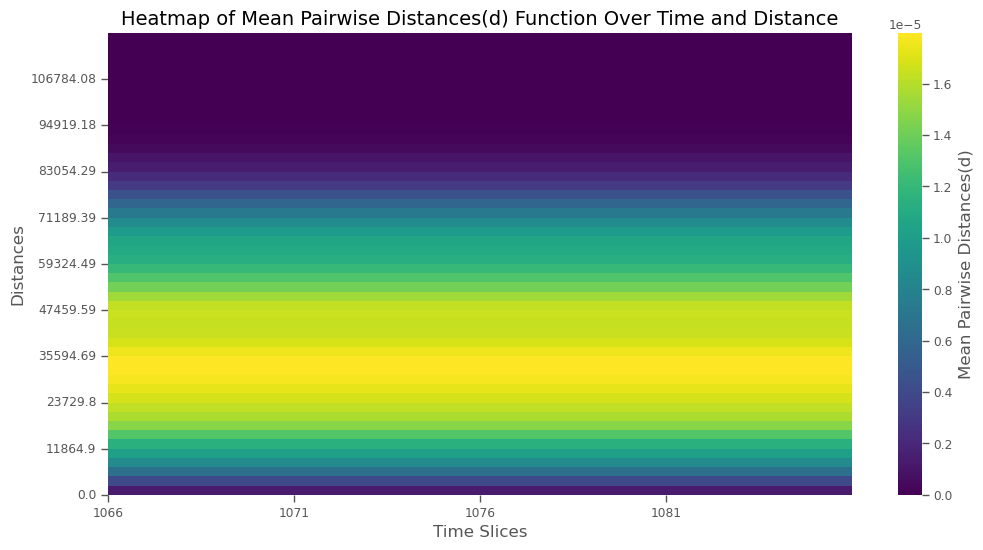
\includegraphics{analysis_files/figure-pdf/cell-27-output-2.png}

\paragraph{Complete Spatial
Randomness}\label{complete-spatial-randomness-1}

\paragraph{Figure S13: Heatmap of PDD versus Time of CSR for
Hampshire}\label{figure-s13-heatmap-of-pdd-versus-time-of-csr-for-hampshire}

\begin{Shaded}
\begin{Highlighting}[]
\CommentTok{\# Get MC iterations for incorporating chronological uncertainty and CSR}
\NormalTok{csr\_simulations\_ham }\OperatorTok{=}\NormalTok{ clustering.mc\_samples(}
\NormalTok{    doomsday\_points, }
\NormalTok{    time\_slices }\OperatorTok{=}\NormalTok{ time\_slices\_ham,  }
\NormalTok{    num\_iterations }\OperatorTok{=}\NormalTok{ num\_iterations,}
\NormalTok{    null\_model }\OperatorTok{=}\NormalTok{ clustering.csr\_sample,}
\NormalTok{    x\_min }\OperatorTok{=}\NormalTok{ x\_min, }
\NormalTok{    x\_max }\OperatorTok{=}\NormalTok{ x\_max,}
\NormalTok{    y\_min }\OperatorTok{=}\NormalTok{ y\_min, }
\NormalTok{    y\_max }\OperatorTok{=}\NormalTok{ y\_max}
\NormalTok{)}

\CommentTok{\# Calulate the pairwise distances for the CSR sample}
\NormalTok{csr\_pairwise\_density\_ham, csr\_support\_ham }\OperatorTok{=}\NormalTok{ clustering.temporal\_pairwise(}
\NormalTok{    csr\_simulations\_ham, }
\NormalTok{    time\_slices\_ham, }
\NormalTok{    bw }\OperatorTok{=}\NormalTok{ pair\_bw, }
\NormalTok{    use\_kde }\OperatorTok{=}\NormalTok{ use\_kde,}
\NormalTok{    kde\_sample\_n }\OperatorTok{=}\NormalTok{ kde\_sample\_n, }
\NormalTok{    max\_distance }\OperatorTok{=}\NormalTok{ max\_distance,}
\NormalTok{    kde\_custom }\OperatorTok{=}\NormalTok{ kde\_custom}
\NormalTok{)}

\CommentTok{\# Visualize clustering with heatmap}
\NormalTok{clustering\_heatmap(}
\NormalTok{    csr\_pairwise\_density\_ham,}
\NormalTok{    csr\_support\_ham,}
\NormalTok{    time\_slices\_ham,}
\NormalTok{    result\_type }\OperatorTok{=} \StringTok{\textquotesingle{}Pairwise Distances\textquotesingle{}}
\NormalTok{)}
\end{Highlighting}
\end{Shaded}

\begin{verbatim}
(<Figure size 1200x600 with 2 Axes>,
 <Axes: title={'center': 'Heatmap of Mean Pairwise Distances(d) Function Over Time and Distance'}, xlabel='Time Slices', ylabel='Distances'>)
\end{verbatim}

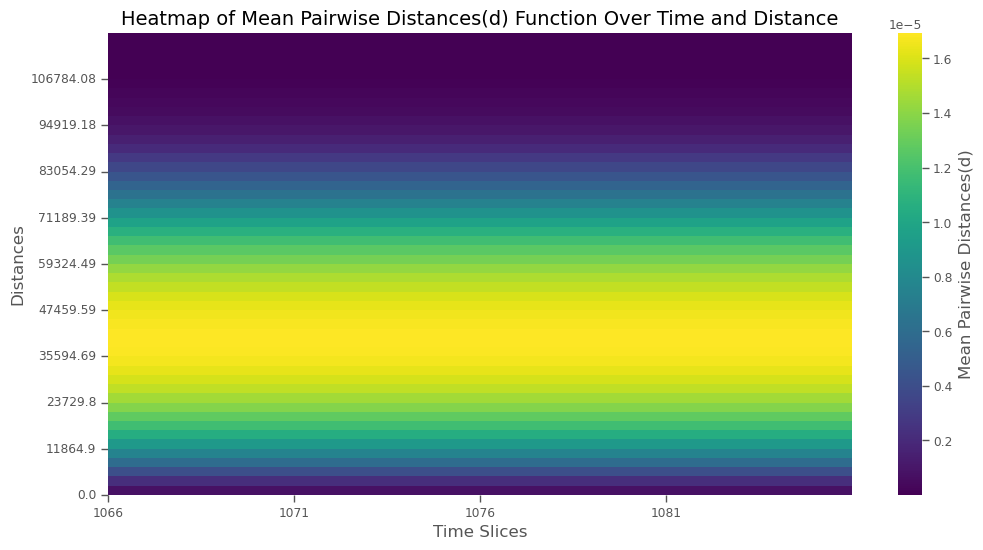
\includegraphics{analysis_files/figure-pdf/cell-28-output-2.png}

\paragraph{Baseline-Informed Spatial
Expectation}\label{baseline-informed-spatial-expectation-1}

\paragraph{Figure S14: Heatmap of PDD Statistical Significance compred
to BISE for
Hampshire}\label{figure-s14-heatmap-of-pdd-statistical-significance-compred-to-bise-for-hampshire}

\begin{Shaded}
\begin{Highlighting}[]
\CommentTok{\# Get MC iterations for incorporating chronological uncertainty with BISE}
\NormalTok{bise\_simulations\_ham }\OperatorTok{=}\NormalTok{ clustering.mc\_samples(}
\NormalTok{    doomsday\_points, }
\NormalTok{    time\_slices\_ham, }
\NormalTok{    num\_iterations}\OperatorTok{=}\NormalTok{num\_iterations,}
\NormalTok{    null\_model}\OperatorTok{=}\NormalTok{clustering.bise}
\NormalTok{)}

\CommentTok{\# Calulate the pairwise distances for the LISE sample}
\NormalTok{bise\_pairwise\_density\_ham, bise\_support\_ham }\OperatorTok{=}\NormalTok{ clustering.temporal\_pairwise(}
\NormalTok{    bise\_simulations\_ham, }
\NormalTok{    time\_slices\_ham, }
\NormalTok{    bw }\OperatorTok{=}\NormalTok{ pair\_bw, }
\NormalTok{    use\_kde }\OperatorTok{=}\NormalTok{ use\_kde,}
\NormalTok{    kde\_sample\_n}\OperatorTok{=}\NormalTok{kde\_sample\_n, }
\NormalTok{    max\_distance }\OperatorTok{=}\NormalTok{ max\_distance,}
\NormalTok{    kde\_custom}\OperatorTok{=}\NormalTok{kde\_custom}
\NormalTok{)}

\CommentTok{\# Calculate the p{-}values for density differences between }
\CommentTok{\# the observed points and the simulated CSR baseline per }
\CommentTok{\# distance and temporal slice}
\NormalTok{p\_diff\_array\_bise\_ham, diff\_array\_bise\_ham }\OperatorTok{=}\NormalTok{ clustering.p\_diff(}
\NormalTok{    pairwise\_density\_ham, }
\NormalTok{    bise\_pairwise\_density\_ham}
\NormalTok{)}

\CommentTok{\# Plot the heatmap of probabilities}
\NormalTok{pdiff\_heatmap(}
\NormalTok{    p\_diff\_array\_bise\_ham,}
\NormalTok{    time\_slices\_ham,}
\NormalTok{    bise\_support\_ham}
\NormalTok{)}
\end{Highlighting}
\end{Shaded}

\begin{verbatim}
(<Figure size 1200x600 with 2 Axes>,
 <Axes: title={'center': 'Probability Heat Map'}, xlabel='Time Slices', ylabel='Pairwise Distances'>)
\end{verbatim}

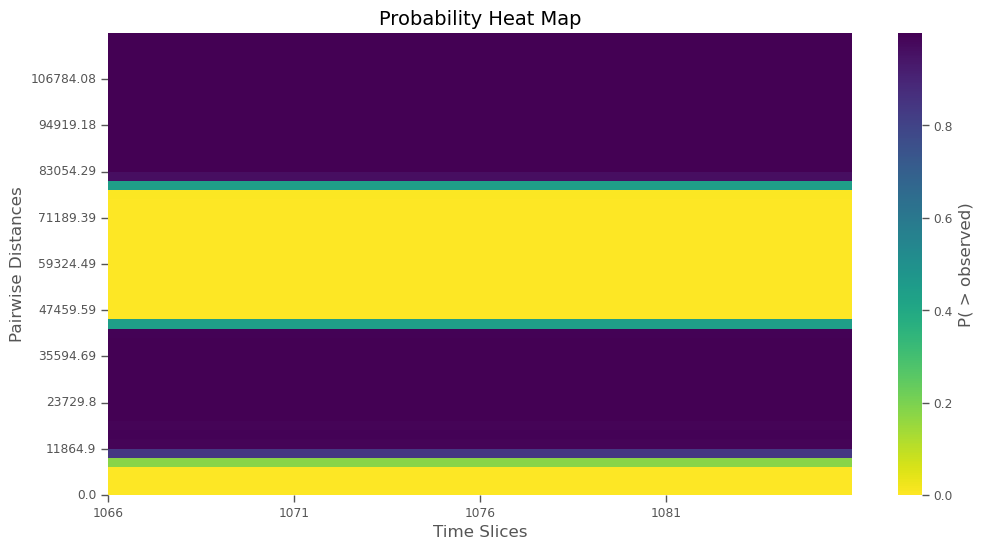
\includegraphics{analysis_files/figure-pdf/cell-29-output-2.png}

\paragraph{One Time Slice}\label{one-time-slice-1}

\paragraph{Figure S15: PDD of Hampshire Estates compared to CSR and BISE
Null Models at 1066
CE}\label{figure-s15-pdd-of-hampshire-estates-compared-to-csr-and-bise-null-models-at-1066-ce}

\begin{Shaded}
\begin{Highlighting}[]
\CommentTok{\#from chronocluster.utils import plot\_pdd}
\NormalTok{time\_slice\_idx }\OperatorTok{=}\NormalTok{ np.where(time\_slices\_ham }\OperatorTok{==} \DecValTok{1066}\NormalTok{)[}\DecValTok{0}\NormalTok{][}\DecValTok{0}\NormalTok{]}

\CommentTok{\# List of density arrays}
\NormalTok{density\_arrays }\OperatorTok{=}\NormalTok{ [}
\NormalTok{    pairwise\_density\_ham, }
\NormalTok{    csr\_pairwise\_density\_ham, }
\NormalTok{    bise\_pairwise\_density\_ham]}

\CommentTok{\# Generate the plot and get the figure and axis objects}
\NormalTok{fig, ax }\OperatorTok{=}\NormalTok{ plot\_pdd(}
\NormalTok{    time\_slices}\OperatorTok{=}\NormalTok{time\_slices\_ham,}
\NormalTok{    time\_slice\_idx}\OperatorTok{=}\NormalTok{time\_slice\_idx,}
\NormalTok{    support}\OperatorTok{=}\NormalTok{support\_ham,}
\NormalTok{    density\_arrays}\OperatorTok{=}\NormalTok{density\_arrays,}
\NormalTok{    quantiles}\OperatorTok{=}\NormalTok{[}\FloatTok{0.025}\NormalTok{, }\FloatTok{0.975}\NormalTok{],}
\NormalTok{    density\_names}\OperatorTok{=}\NormalTok{[}\StringTok{"Empirical"}\NormalTok{, }\StringTok{"CSR"}\NormalTok{, }\StringTok{"BISE"}\NormalTok{],}
\NormalTok{    colors}\OperatorTok{=}\NormalTok{[}\StringTok{"blue"}\NormalTok{, }\StringTok{"orange"}\NormalTok{, }\StringTok{"green"}\NormalTok{]}
\NormalTok{)}

\NormalTok{ax.set\_title(}\StringTok{"PDD Hampshire 1066 CE"}\NormalTok{)}

\CommentTok{\# Get current tick positions and convert labels to km}
\NormalTok{x\_ticks }\OperatorTok{=}\NormalTok{ ax.get\_xticks()}
\NormalTok{ax.set\_xticklabels(np.}\BuiltInTok{round}\NormalTok{(x\_ticks }\OperatorTok{/} \DecValTok{1000}\NormalTok{, }\DecValTok{1}\NormalTok{))  }\CommentTok{\# e.g. 1000 → 1.0 km}

\CommentTok{\# Update axis label}
\NormalTok{ax.set\_xlabel(}\StringTok{"Distance (km)"}\NormalTok{)}

\CommentTok{\# Show the plot}
\NormalTok{plt.show()}

\NormalTok{fig.savefig(}
    \StringTok{"../Output/pdd\_null\_hampshire.png"}\NormalTok{, }
\NormalTok{    dpi }\OperatorTok{=} \DecValTok{300}\NormalTok{, }
\NormalTok{    bbox\_inches }\OperatorTok{=} \StringTok{"tight"}
\NormalTok{)}
\NormalTok{fig.savefig(}
    \StringTok{"../Output/pdd\_null\_hampshire.svg"}\NormalTok{, }
\NormalTok{    bbox\_inches }\OperatorTok{=} \StringTok{"tight"}
\NormalTok{)}
\end{Highlighting}
\end{Shaded}

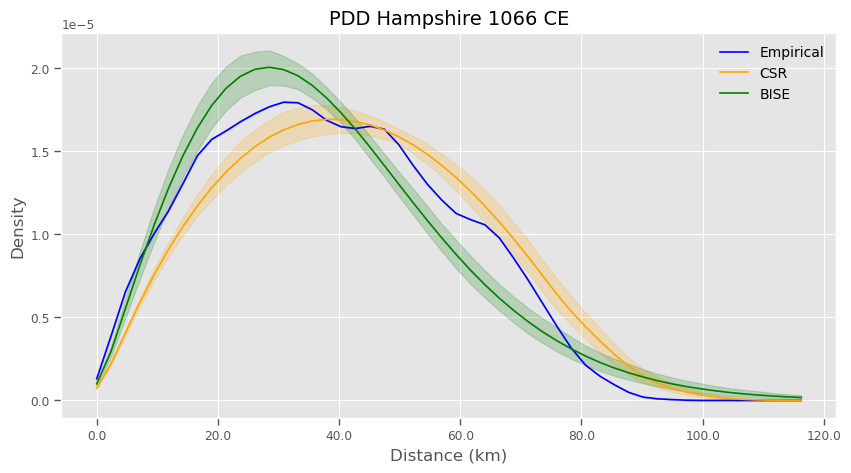
\includegraphics{analysis_files/figure-pdf/cell-30-output-1.png}

\paragraph{Figure S16: Difference between PDD and BISE Null Model for
Hampshire's Estates at 1066
CE}\label{figure-s16-difference-between-pdd-and-bise-null-model-for-hampshires-estates-at-1066-ce}

\begin{Shaded}
\begin{Highlighting}[]
\CommentTok{\# List of density arrays}
\NormalTok{density\_arrays }\OperatorTok{=}\NormalTok{ [diff\_array\_bise\_ham]}

\CommentTok{\# Generate the plot and get the figure and axis objects}
\NormalTok{fig, ax }\OperatorTok{=}\NormalTok{ plot\_pdd(}
\NormalTok{    time\_slices}\OperatorTok{=}\NormalTok{time\_slices\_ham,}
\NormalTok{    time\_slice\_idx}\OperatorTok{=}\NormalTok{time\_slice\_idx,}
\NormalTok{    support}\OperatorTok{=}\NormalTok{support\_ham,}
\NormalTok{    density\_arrays}\OperatorTok{=}\NormalTok{density\_arrays,}
\NormalTok{    quantiles}\OperatorTok{=}\NormalTok{[}\FloatTok{0.025}\NormalTok{, }\FloatTok{0.975}\NormalTok{],}
\NormalTok{    density\_names}\OperatorTok{=}\NormalTok{[}\StringTok{"$\textbackslash{}Delta$PDD"}\NormalTok{],}
\NormalTok{    colors}\OperatorTok{=}\NormalTok{[}\StringTok{"blue"}\NormalTok{]}
\NormalTok{)}

\CommentTok{\# Add a horizontal line at y=0}
\NormalTok{ax.axhline(y}\OperatorTok{=}\DecValTok{0}\NormalTok{, color}\OperatorTok{=}\StringTok{\textquotesingle{}red\textquotesingle{}}\NormalTok{, linestyle}\OperatorTok{=}\StringTok{\textquotesingle{}{-}{-}\textquotesingle{}}\NormalTok{, linewidth}\OperatorTok{=}\FloatTok{1.5}\NormalTok{)}

\NormalTok{ax.set\_title(}\StringTok{"$\textbackslash{}Delta$PDD Hampshire 1066 CE"}\NormalTok{)}
\CommentTok{\#ax.set\_xlabel("Distance (m)")}

\CommentTok{\# Get current tick positions and convert labels to km}
\NormalTok{x\_ticks }\OperatorTok{=}\NormalTok{ ax.get\_xticks()}
\NormalTok{ax.set\_xticklabels(np.}\BuiltInTok{round}\NormalTok{(x\_ticks }\OperatorTok{/} \DecValTok{1000}\NormalTok{, }\DecValTok{1}\NormalTok{))  }\CommentTok{\# e.g. 1000 → 1.0 km}

\CommentTok{\# Update axis label}
\NormalTok{ax.set\_xlabel(}\StringTok{"Distance (km)"}\NormalTok{)}

\CommentTok{\# Show the plot}
\NormalTok{plt.show()}
\end{Highlighting}
\end{Shaded}

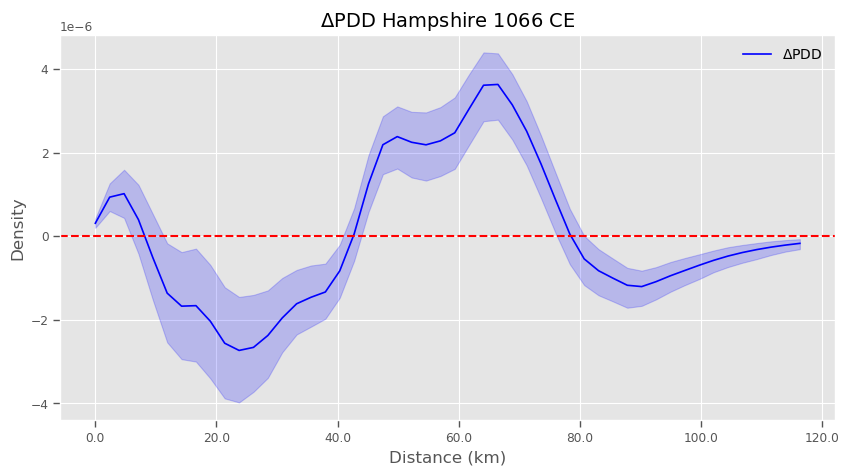
\includegraphics{analysis_files/figure-pdf/cell-31-output-1.png}

\paragraph{\texorpdfstring{Figure S17: \(\Delta\) PDDs of Angkor and
Hampshire Side by
Side}{Figure S17: \textbackslash Delta PDDs of Angkor and Hampshire Side by Side}}\label{figure-s17-delta-pdds-of-angkor-and-hampshire-side-by-side}

\begin{Shaded}
\begin{Highlighting}[]
\CommentTok{\# Create a figure with two side{-}by{-}side subplots}
\NormalTok{fig, (ax1, ax2) }\OperatorTok{=}\NormalTok{ plt.subplots(}\DecValTok{1}\NormalTok{, }\DecValTok{2}\NormalTok{, figsize}\OperatorTok{=}\NormalTok{(}\DecValTok{12}\NormalTok{, }\DecValTok{5}\NormalTok{), sharex}\OperatorTok{=}\VariableTok{False}\NormalTok{, sharey}\OperatorTok{=}\VariableTok{True}\NormalTok{)}

\CommentTok{\# First plot, Angkor}
\NormalTok{time\_slice\_idx }\OperatorTok{=}\NormalTok{ np.where(time\_slices }\OperatorTok{==} \DecValTok{1000}\NormalTok{)[}\DecValTok{0}\NormalTok{][}\DecValTok{0}\NormalTok{]}
\NormalTok{plot\_pdd(}
\NormalTok{    time\_slices }\OperatorTok{=}\NormalTok{ time\_slices,}
\NormalTok{    time\_slice\_idx }\OperatorTok{=}\NormalTok{ time\_slice\_idx,}
\NormalTok{    support }\OperatorTok{=}\NormalTok{ support\_angkor,}
\NormalTok{    density\_arrays }\OperatorTok{=}\NormalTok{ [diff\_array\_bise\_angkor],}
\NormalTok{    quantiles }\OperatorTok{=}\NormalTok{ [}\FloatTok{0.025}\NormalTok{, }\FloatTok{0.975}\NormalTok{],}
\NormalTok{    density\_names }\OperatorTok{=}\NormalTok{ [}\StringTok{"$\textbackslash{}Delta$PDD Angkor"}\NormalTok{],}
\NormalTok{    colors }\OperatorTok{=}\NormalTok{ [}\StringTok{"blue"}\NormalTok{],}
\NormalTok{    ax}\OperatorTok{=}\NormalTok{ax1}
\NormalTok{)}
\NormalTok{ax1.axhline(y}\OperatorTok{=}\DecValTok{0}\NormalTok{, color}\OperatorTok{=}\StringTok{\textquotesingle{}red\textquotesingle{}}\NormalTok{, linestyle}\OperatorTok{=}\StringTok{\textquotesingle{}{-}{-}\textquotesingle{}}\NormalTok{, linewidth}\OperatorTok{=}\FloatTok{1.5}\NormalTok{)}
\NormalTok{ax1.set\_title(}\StringTok{"$\textbackslash{}Delta$PDD Angkor"}\NormalTok{)}
\CommentTok{\#ax1.set\_xlabel("Distance (m)")}

\CommentTok{\# Get current tick positions and convert labels to km}
\NormalTok{x\_ticks }\OperatorTok{=}\NormalTok{ ax1.get\_xticks()}
\NormalTok{ax1.set\_xticklabels(np.}\BuiltInTok{round}\NormalTok{(x\_ticks }\OperatorTok{/} \DecValTok{1000}\NormalTok{, }\DecValTok{1}\NormalTok{))  }\CommentTok{\# e.g. 1000 → 1.0 km}

\CommentTok{\# Update axis label}
\NormalTok{ax1.set\_xlabel(}\StringTok{"Distance (km)"}\NormalTok{)}

\CommentTok{\# Second plot, Hampshire}
\NormalTok{time\_slice\_idx }\OperatorTok{=}\NormalTok{ np.where(time\_slices\_ham }\OperatorTok{==} \DecValTok{1066}\NormalTok{)[}\DecValTok{0}\NormalTok{][}\DecValTok{0}\NormalTok{]}
\NormalTok{plot\_pdd(}
\NormalTok{    time\_slices }\OperatorTok{=}\NormalTok{ time\_slices\_ham,}
\NormalTok{    time\_slice\_idx }\OperatorTok{=}\NormalTok{ time\_slice\_idx,}
\NormalTok{    support }\OperatorTok{=}\NormalTok{ support\_ham,}
\NormalTok{    density\_arrays }\OperatorTok{=}\NormalTok{ [diff\_array\_bise\_ham],}
\NormalTok{    quantiles }\OperatorTok{=}\NormalTok{ [}\FloatTok{0.025}\NormalTok{, }\FloatTok{0.975}\NormalTok{],}
\NormalTok{    density\_names }\OperatorTok{=}\NormalTok{ [}\StringTok{"$\textbackslash{}Delta$PDD Hampshire"}\NormalTok{],}
\NormalTok{    colors }\OperatorTok{=}\NormalTok{ [}\StringTok{"green"}\NormalTok{],}
\NormalTok{    ax}\OperatorTok{=}\NormalTok{ax2}
\NormalTok{)}
\NormalTok{ax2.axhline(y}\OperatorTok{=}\DecValTok{0}\NormalTok{, color}\OperatorTok{=}\StringTok{\textquotesingle{}red\textquotesingle{}}\NormalTok{, linestyle}\OperatorTok{=}\StringTok{\textquotesingle{}{-}{-}\textquotesingle{}}\NormalTok{, linewidth}\OperatorTok{=}\FloatTok{1.5}\NormalTok{)}
\NormalTok{ax2.set\_title(}\StringTok{"$\textbackslash{}Delta$PDD Hampshire"}\NormalTok{)}
\CommentTok{\#ax2.set\_xlabel("Distance (m)")}

\CommentTok{\# Get current tick positions and convert labels to km}
\NormalTok{x\_ticks }\OperatorTok{=}\NormalTok{ ax2.get\_xticks()}
\NormalTok{ax2.set\_xticklabels(np.}\BuiltInTok{round}\NormalTok{(x\_ticks }\OperatorTok{/} \DecValTok{1000}\NormalTok{, }\DecValTok{1}\NormalTok{))  }\CommentTok{\# e.g. 1000 → 1.0 km}

\CommentTok{\# Update axis label}
\NormalTok{ax2.set\_xlabel(}\StringTok{"Distance (km)"}\NormalTok{)}

\CommentTok{\# Adjust layout and show the combined plot}
\NormalTok{plt.tight\_layout()}
\NormalTok{plt.show()}

\NormalTok{fig.savefig(}
    \StringTok{"../Output/dpdd\_compared.png"}\NormalTok{, }
\NormalTok{    dpi }\OperatorTok{=} \DecValTok{300}\NormalTok{, }
\NormalTok{    bbox\_inches }\OperatorTok{=} \StringTok{"tight"}
\NormalTok{)}
\NormalTok{fig.savefig(}
    \StringTok{"../Output/dpdd\_compared.svg"}\NormalTok{, }
\NormalTok{    bbox\_inches }\OperatorTok{=} \StringTok{"tight"}
\NormalTok{)}
\end{Highlighting}
\end{Shaded}

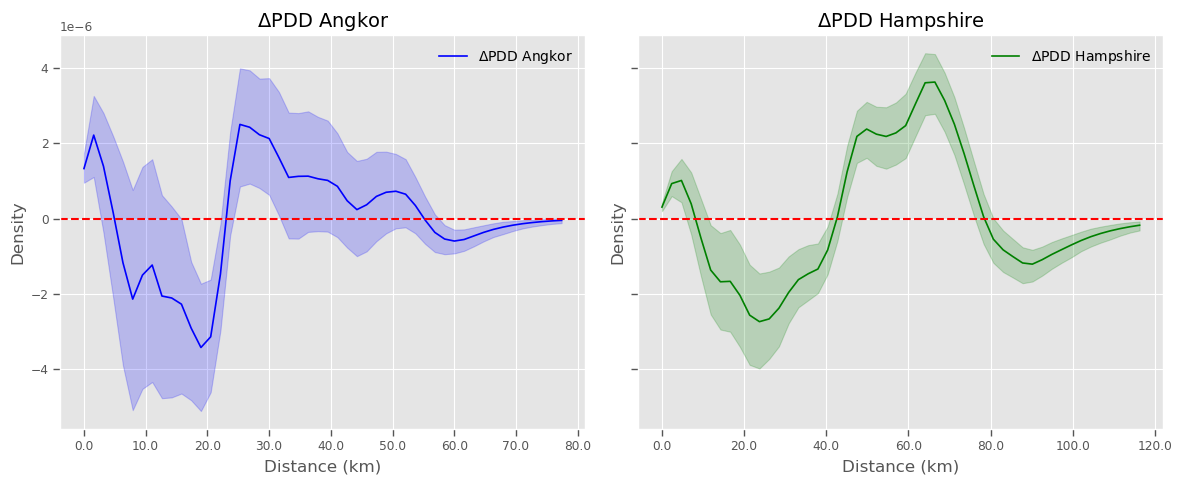
\includegraphics{analysis_files/figure-pdf/cell-32-output-1.png}

\paragraph{\texorpdfstring{Figure S18: \(\Delta\) PDDs compared with
Angkor's PDD
Scaled}{Figure S18: \textbackslash Delta PDDs compared with Angkor's PDD Scaled}}\label{figure-s18-delta-pdds-compared-with-angkors-pdd-scaled}

\begin{Shaded}
\begin{Highlighting}[]
\ImportTok{import}\NormalTok{ numpy }\ImportTok{as}\NormalTok{ np}
\ImportTok{import}\NormalTok{ matplotlib.pyplot }\ImportTok{as}\NormalTok{ plt}

\CommentTok{\# Scaling ratio for Angkor x{-}axis}
\NormalTok{scaling\_ratio }\OperatorTok{=} \FloatTok{1.5}
\NormalTok{scaled\_support\_angkor }\OperatorTok{=}\NormalTok{ np.array(support\_angkor) }\OperatorTok{*}\NormalTok{ scaling\_ratio}

\CommentTok{\# Create a vertically stacked figure with shared x{-}axis}
\NormalTok{fig, (ax1, ax2) }\OperatorTok{=}\NormalTok{ plt.subplots(}
    \DecValTok{2}\NormalTok{, }\DecValTok{1}\NormalTok{,}
\NormalTok{    figsize}\OperatorTok{=}\NormalTok{(}\DecValTok{10}\NormalTok{, }\DecValTok{8}\NormalTok{),}
\NormalTok{    sharex}\OperatorTok{=}\VariableTok{True}\NormalTok{,}
\NormalTok{    gridspec\_kw}\OperatorTok{=}\NormalTok{\{}\StringTok{\textquotesingle{}height\_ratios\textquotesingle{}}\NormalTok{: [}\DecValTok{1}\NormalTok{, }\DecValTok{1}\NormalTok{]\}}
\NormalTok{)}

\CommentTok{\# First plot: Angkor (scaled x{-}axis)}
\NormalTok{time\_slice\_idx\_angkor }\OperatorTok{=}\NormalTok{ np.where(time\_slices }\OperatorTok{==} \DecValTok{1000}\NormalTok{)[}\DecValTok{0}\NormalTok{][}\DecValTok{0}\NormalTok{]}
\NormalTok{plot\_pdd(}
\NormalTok{    time\_slices}\OperatorTok{=}\NormalTok{time\_slices,}
\NormalTok{    time\_slice\_idx}\OperatorTok{=}\NormalTok{time\_slice\_idx\_angkor,}
\NormalTok{    support}\OperatorTok{=}\NormalTok{scaled\_support\_angkor,}
\NormalTok{    density\_arrays}\OperatorTok{=}\NormalTok{[diff\_array\_bise\_angkor],}
\NormalTok{    quantiles}\OperatorTok{=}\NormalTok{[}\FloatTok{0.025}\NormalTok{, }\FloatTok{0.975}\NormalTok{],}
\NormalTok{    density\_names}\OperatorTok{=}\NormalTok{[}\StringTok{"$\textbackslash{}Delta$PDD Angkor"}\NormalTok{],}
\NormalTok{    colors}\OperatorTok{=}\NormalTok{[}\StringTok{"blue"}\NormalTok{],}
\NormalTok{    ax}\OperatorTok{=}\NormalTok{ax1}
\NormalTok{)}
\NormalTok{ax1.set\_title(}\StringTok{"$\textbackslash{}Delta$PDD Angkor (Scaled)"}\NormalTok{)}
\NormalTok{ax1.tick\_params(labelbottom}\OperatorTok{=}\VariableTok{False}\NormalTok{)}
\CommentTok{\#ax1.set\_xlabel("Distance (m)")}

\CommentTok{\# Get current tick positions and convert labels to km}
\NormalTok{x\_ticks }\OperatorTok{=}\NormalTok{ ax1.get\_xticks()}
\NormalTok{ax1.set\_xticklabels(np.}\BuiltInTok{round}\NormalTok{(x\_ticks }\OperatorTok{/} \DecValTok{1000}\NormalTok{, }\DecValTok{1}\NormalTok{))  }\CommentTok{\# e.g. 1000 → 1.0 km}

\CommentTok{\# Update axis label}
\NormalTok{ax1.set\_xlabel(}\StringTok{"Distance (km)"}\NormalTok{)}

\CommentTok{\# Second plot: Hampshire}
\NormalTok{time\_slice\_idx\_ham }\OperatorTok{=}\NormalTok{ np.where(time\_slices\_ham }\OperatorTok{==} \DecValTok{1066}\NormalTok{)[}\DecValTok{0}\NormalTok{][}\DecValTok{0}\NormalTok{]}
\NormalTok{plot\_pdd(}
\NormalTok{    time\_slices }\OperatorTok{=}\NormalTok{ time\_slices\_ham,}
\NormalTok{    time\_slice\_idx }\OperatorTok{=}\NormalTok{ time\_slice\_idx\_ham,}
\NormalTok{    support }\OperatorTok{=}\NormalTok{ support\_ham,}
\NormalTok{    density\_arrays }\OperatorTok{=}\NormalTok{ [diff\_array\_bise\_ham],}
\NormalTok{    quantiles }\OperatorTok{=}\NormalTok{ [}\FloatTok{0.025}\NormalTok{, }\FloatTok{0.975}\NormalTok{],}
\NormalTok{    density\_names }\OperatorTok{=}\NormalTok{ [}\StringTok{"$\textbackslash{}Delta$PDD Hampshire"}\NormalTok{],}
\NormalTok{    colors }\OperatorTok{=}\NormalTok{ [}\StringTok{"green"}\NormalTok{],}
\NormalTok{    ax}\OperatorTok{=}\NormalTok{ax2}
\NormalTok{)}
\NormalTok{ax2.set\_title(}\StringTok{"$\textbackslash{}Delta$PDD Hampshire"}\NormalTok{)}
\CommentTok{\#ax2.set\_xlabel("Distance (m)")}

\CommentTok{\# Get current tick positions and convert labels to km}
\NormalTok{x\_ticks }\OperatorTok{=}\NormalTok{ ax2.get\_xticks()}
\NormalTok{ax2.set\_xticklabels(np.}\BuiltInTok{round}\NormalTok{(x\_ticks }\OperatorTok{/} \DecValTok{1000}\NormalTok{, }\DecValTok{1}\NormalTok{))  }\CommentTok{\# e.g. 1000 → 1.0 km}

\CommentTok{\# Update axis label}
\NormalTok{ax2.set\_xlabel(}\StringTok{"Distance (km)"}\NormalTok{)}

\CommentTok{\# Final layout tweaks}
\NormalTok{plt.tight\_layout()}
\NormalTok{plt.show()}

\NormalTok{fig.savefig(}
    \StringTok{"../Output/dpdd\_scaled.png"}\NormalTok{, }
\NormalTok{    dpi}\OperatorTok{=}\DecValTok{300}\NormalTok{, }
\NormalTok{    bbox\_inches}\OperatorTok{=}\StringTok{"tight"}
\NormalTok{)}
\NormalTok{fig.savefig(}
    \StringTok{"../Output/dpdd\_scaled.svg"}\NormalTok{, }
\NormalTok{    bbox\_inches}\OperatorTok{=}\StringTok{"tight"}
\NormalTok{)}
\end{Highlighting}
\end{Shaded}

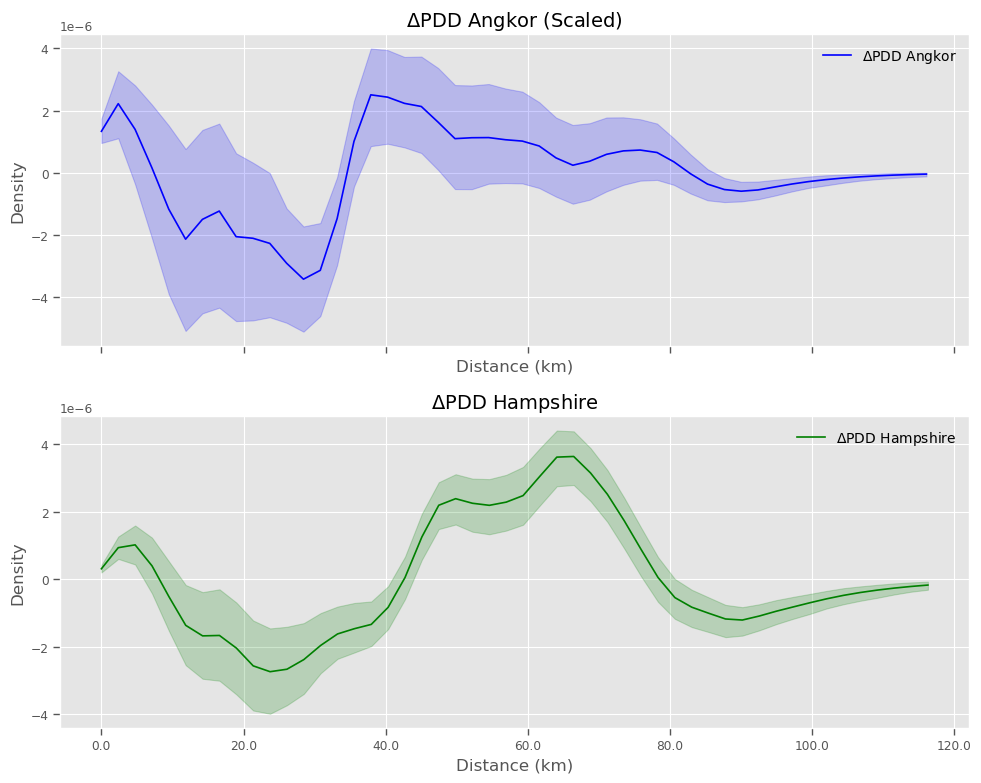
\includegraphics{analysis_files/figure-pdf/cell-33-output-1.png}

\subsection{First Peaks}\label{first-peaks}

\begin{Shaded}
\begin{Highlighting}[]
\ImportTok{from}\NormalTok{ scipy.signal }\ImportTok{import}\NormalTok{ find\_peaks}
\ImportTok{import}\NormalTok{ warnings}

\KeywordTok{def}\NormalTok{ find\_first\_peak(pdd\_slice, support):}
    \CommentTok{"""}
\CommentTok{    Finds the first peak in a PDD slice.}

\CommentTok{    Parameters:}
\CommentTok{    {-}{-}{-}{-}{-}{-}{-}{-}{-}{-}{-}}
\CommentTok{    pdd\_slice : np.ndarray}
\CommentTok{        A 1D array of PDD values for a single realization.}
\CommentTok{    support : np.ndarray}
\CommentTok{        Array of distance values (x{-}axis).}

\CommentTok{    Returns:}
\CommentTok{    {-}{-}{-}{-}{-}{-}{-}{-}}
\CommentTok{    float}
\CommentTok{        Distance (x{-}coordinate) of the first peak.}
\CommentTok{    """}
    \CommentTok{\# Find all peaks in the PDD slice}
\NormalTok{    peaks, \_ }\OperatorTok{=}\NormalTok{ find\_peaks(pdd\_slice)}

    \CommentTok{\# If peaks exist, return the first one}
    \ControlFlowTok{if} \BuiltInTok{len}\NormalTok{(peaks) }\OperatorTok{\textgreater{}} \DecValTok{0}\NormalTok{:}
        \ControlFlowTok{return}\NormalTok{ support[peaks[}\DecValTok{0}\NormalTok{]]}

    \CommentTok{\# If no peaks are found, return NaN}
    \ControlFlowTok{return}\NormalTok{ np.nan}

\KeywordTok{def}\NormalTok{ find\_all\_first\_peaks(diff\_array, support, time\_slice\_idx):}
    \CommentTok{"""}
\CommentTok{    Finds the first peak for all realizations in a PDD difference array and returns }
\CommentTok{    both the peak locations and their corresponding densities.}

\CommentTok{    Parameters:}
\CommentTok{    {-}{-}{-}{-}{-}{-}{-}{-}{-}{-}{-}}
\CommentTok{    diff\_array : np.ndarray}
\CommentTok{        3D array of PDD difference values (distances x time\_slices x realizations).}
\CommentTok{    support : np.ndarray}
\CommentTok{        Array of distance values (x{-}axis).}
\CommentTok{    time\_slice\_idx : int}
\CommentTok{        Index of the time slice to analyze.}

\CommentTok{    Returns:}
\CommentTok{    {-}{-}{-}{-}{-}{-}{-}{-}}
\CommentTok{    peaks : list}
\CommentTok{        List of first peak locations for all realizations.}
\CommentTok{    densities : list}
\CommentTok{        List of density values at the first peak for all realizations.}
\CommentTok{    """}
\NormalTok{    peaks }\OperatorTok{=}\NormalTok{ []}
\NormalTok{    densities }\OperatorTok{=}\NormalTok{ []}
\NormalTok{    num\_realizations }\OperatorTok{=}\NormalTok{ diff\_array.shape[}\DecValTok{2}\NormalTok{]}

    \ControlFlowTok{for}\NormalTok{ realization\_idx }\KeywordTok{in} \BuiltInTok{range}\NormalTok{(num\_realizations):}
        \CommentTok{\# Extract the PDD slice for the current realization}
\NormalTok{        pdd\_slice }\OperatorTok{=}\NormalTok{ diff\_array[:, time\_slice\_idx, realization\_idx]}

        \CommentTok{\# Find the first peak location}
\NormalTok{        peak\_location }\OperatorTok{=}\NormalTok{ find\_first\_peak(pdd\_slice, support)}
        
        \CommentTok{\# if no peak, just return nan}
        \ControlFlowTok{if}\NormalTok{ np.isnan(peak\_location):}
\NormalTok{            warnings.warn(}\StringTok{"No peak found."}\NormalTok{, }\PreprocessorTok{UserWarning}\NormalTok{)}
\NormalTok{            peaks.append(np.nan)}
\NormalTok{            densities.append(np.nan)}
        \ControlFlowTok{else}\NormalTok{:}
            \CommentTok{\# Get the density value at the peak}
\NormalTok{            peak\_density }\OperatorTok{=}\NormalTok{ pdd\_slice[support }\OperatorTok{==}\NormalTok{ peak\_location][}\DecValTok{0}\NormalTok{]}

            \CommentTok{\# Append results}
\NormalTok{            peaks.append(peak\_location)}
\NormalTok{            densities.append(peak\_density)}

    \ControlFlowTok{return}\NormalTok{ np.array(peaks), np.array(densities)}
\end{Highlighting}
\end{Shaded}

\subsubsection{Set Common Parameters}\label{set-common-parameters}

\begin{Shaded}
\begin{Highlighting}[]
\NormalTok{num\_iterations }\OperatorTok{=} \DecValTok{500}
\NormalTok{use\_kde }\OperatorTok{=} \VariableTok{True}
\NormalTok{pair\_bw }\OperatorTok{=} \VariableTok{None}
\NormalTok{kde\_sample\_n }\OperatorTok{=} \DecValTok{100}
\NormalTok{kde\_custom}\OperatorTok{=}\NormalTok{cuml\_kde}
\NormalTok{max\_distance }\OperatorTok{=} \DecValTok{15000}
\end{Highlighting}
\end{Shaded}

\subsubsection{Angkor First Peak}\label{angkor-first-peak}

\begin{Shaded}
\begin{Highlighting}[]
\NormalTok{time\_slice }\OperatorTok{=} \DecValTok{1100}

\CommentTok{\# Run the Monte Carlo simulation to get an ensemble of probable }
\CommentTok{\# lists of points included in each time slice.}
\NormalTok{simulations }\OperatorTok{=}\NormalTok{ clustering.mc\_samples(}
\NormalTok{    points, }
\NormalTok{    time\_slices}\OperatorTok{=}\NormalTok{[time\_slice],  }
\NormalTok{    num\_iterations}\OperatorTok{=}\NormalTok{num\_iterations}
\NormalTok{)}

\CommentTok{\# Produce pairwise distances to explore clustering structure}
\NormalTok{pairwise\_density\_angkor, support\_angkor }\OperatorTok{=}\NormalTok{ clustering.temporal\_pairwise(}
\NormalTok{    simulations, }
\NormalTok{    [time\_slice],}
\NormalTok{    bw}\OperatorTok{=}\NormalTok{pair\_bw, }
\NormalTok{    use\_kde}\OperatorTok{=}\NormalTok{use\_kde, }
\NormalTok{    kde\_sample\_n}\OperatorTok{=}\NormalTok{kde\_sample\_n,}
\NormalTok{    max\_distance}\OperatorTok{=}\NormalTok{max\_distance,}
\NormalTok{    kde\_custom}\OperatorTok{=}\NormalTok{kde\_custom}
\NormalTok{)}

\CommentTok{\# Get MC iterations for incorporating chronological uncertainty with BISE}
\NormalTok{bise\_simulations }\OperatorTok{=}\NormalTok{ clustering.mc\_samples(}
\NormalTok{    points, }
\NormalTok{    [time\_slice], }
\NormalTok{    num\_iterations}\OperatorTok{=}\NormalTok{num\_iterations,}
\NormalTok{    null\_model}\OperatorTok{=}\NormalTok{clustering.bise}
\NormalTok{)}

\CommentTok{\# Calulate the pairwise distances for the LISE sample}
\NormalTok{bise\_pairwise\_density\_angkor, bise\_support\_angkor }\OperatorTok{=}\NormalTok{ clustering.temporal\_pairwise(}
\NormalTok{    bise\_simulations, }
\NormalTok{    [time\_slice], }
\NormalTok{    bw }\OperatorTok{=}\NormalTok{ pair\_bw, }
\NormalTok{    use\_kde }\OperatorTok{=}\NormalTok{ use\_kde,}
\NormalTok{    kde\_sample\_n}\OperatorTok{=}\NormalTok{kde\_sample\_n, }
\NormalTok{    max\_distance }\OperatorTok{=}\NormalTok{ max\_distance,}
\NormalTok{    kde\_custom}\OperatorTok{=}\NormalTok{kde\_custom}
\NormalTok{)}

\CommentTok{\# Calculate the p{-}values for density differences between the observed points and }
\CommentTok{\# the simulated CSR baseline per distance and temporal slice}
\NormalTok{p\_diff\_array\_angkor, diff\_array\_angkor }\OperatorTok{=}\NormalTok{ clustering.p\_diff(}
\NormalTok{    pairwise\_density\_angkor, }
\NormalTok{    bise\_pairwise\_density\_angkor}
\NormalTok{)}
\end{Highlighting}
\end{Shaded}

\begin{Shaded}
\begin{Highlighting}[]
\NormalTok{p\_pdd\_peaks\_angkor, \_ }\OperatorTok{=}\NormalTok{ find\_all\_first\_peaks(}
\NormalTok{    diff\_array\_angkor, }
\NormalTok{    support\_angkor, }
    \DecValTok{0}
\NormalTok{)}

\CommentTok{\# Convert to a Pandas DataFrame and use describe()}
\NormalTok{summary\_stats }\OperatorTok{=}\NormalTok{ pd.DataFrame(p\_pdd\_peaks\_angkor, columns}\OperatorTok{=}\NormalTok{[}\StringTok{"Values"}\NormalTok{]).describe()}

\CommentTok{\# Display the summary statistics}
\NormalTok{summary\_stats}
\end{Highlighting}
\end{Shaded}

\begin{longtable}[]{@{}ll@{}}
\toprule\noalign{}
& Values \\
\midrule\noalign{}
\endhead
\bottomrule\noalign{}
\endlastfoot
count & 500.000000 \\
mean & 1723.939394 \\
std & 279.623577 \\
min & 909.090909 \\
25\% & 1515.151515 \\
50\% & 1666.666667 \\
75\% & 1969.696970 \\
max & 2878.787879 \\
\end{longtable}

\paragraph{Figure S19: Distribution of First Peak Locations for Angkor
at 1000
CE}\label{figure-s19-distribution-of-first-peak-locations-for-angkor-at-1000-ce}

\begin{Shaded}
\begin{Highlighting}[]
\CommentTok{\# Assuming \textasciigrave{}peaks\textasciigrave{} is your data}
\CommentTok{\# Plot density and rug plot}
\NormalTok{plt.figure(figsize}\OperatorTok{=}\NormalTok{(}\DecValTok{8}\NormalTok{, }\DecValTok{6}\NormalTok{))}
\NormalTok{sns.kdeplot(p\_pdd\_peaks\_angkor, color}\OperatorTok{=}\StringTok{\textquotesingle{}blue\textquotesingle{}}\NormalTok{, label}\OperatorTok{=}\StringTok{"Density"}\NormalTok{)}
\NormalTok{sns.rugplot(p\_pdd\_peaks\_angkor, color}\OperatorTok{=}\StringTok{\textquotesingle{}blue\textquotesingle{}}\NormalTok{, alpha}\OperatorTok{=}\FloatTok{0.5}\NormalTok{)}

\CommentTok{\# Add labels and title}
\NormalTok{plt.xlabel(}\StringTok{"First Peak Location (Distance)"}\NormalTok{)}
\NormalTok{plt.ylabel(}\StringTok{"Density"}\NormalTok{)}
\NormalTok{plt.title(}\SpecialStringTok{f"Distribution of First Peak Locations {-} Angkor at }\SpecialCharTok{\{}\NormalTok{time\_slice}\SpecialCharTok{\}}\SpecialStringTok{"}\NormalTok{)}
\NormalTok{plt.legend()}

\CommentTok{\# Show the plot}
\NormalTok{plt.show()}
\end{Highlighting}
\end{Shaded}

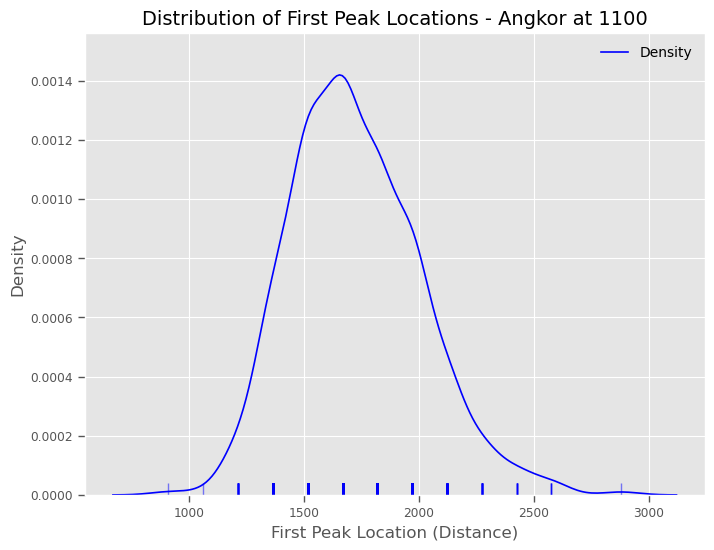
\includegraphics{analysis_files/figure-pdf/cell-38-output-1.png}

\subsubsection{Hampshire First Peak}\label{hampshire-first-peak}

\begin{Shaded}
\begin{Highlighting}[]
\NormalTok{time\_slice }\OperatorTok{=} \DecValTok{1066}

\CommentTok{\# Run the Monte Carlo simulation to get an ensemble of probable }
\CommentTok{\# lists of points included in each time slice.}
\NormalTok{simulations }\OperatorTok{=}\NormalTok{ clustering.mc\_samples(}
\NormalTok{    doomsday\_points, }
\NormalTok{    time\_slices}\OperatorTok{=}\NormalTok{[time\_slice],  }
\NormalTok{    num\_iterations}\OperatorTok{=}\NormalTok{num\_iterations}
\NormalTok{)}

\CommentTok{\# Produce pairwise distances to explore clustering structure}
\NormalTok{pairwise\_density\_hampshire, support\_hampshire }\OperatorTok{=}\NormalTok{ clustering.temporal\_pairwise(}
\NormalTok{    simulations, }
\NormalTok{    [time\_slice],}
\NormalTok{    bw}\OperatorTok{=}\NormalTok{pair\_bw, }
\NormalTok{    use\_kde}\OperatorTok{=}\NormalTok{use\_kde, }
\NormalTok{    kde\_sample\_n}\OperatorTok{=}\NormalTok{kde\_sample\_n,}
\NormalTok{    max\_distance}\OperatorTok{=}\NormalTok{max\_distance,}
\NormalTok{    kde\_custom}\OperatorTok{=}\NormalTok{kde\_custom}
\NormalTok{)}

\CommentTok{\# Get MC iterations for incorporating chronological uncertainty with BISE}
\NormalTok{bise\_simulations }\OperatorTok{=}\NormalTok{ clustering.mc\_samples(}
\NormalTok{    doomsday\_points, }
\NormalTok{    [time\_slice], }
\NormalTok{    num\_iterations}\OperatorTok{=}\NormalTok{num\_iterations,}
\NormalTok{    null\_model}\OperatorTok{=}\NormalTok{clustering.bise}
\NormalTok{)}

\CommentTok{\# Calulate the pairwise distances for the BISE sample}
\NormalTok{bise\_pairwise\_density\_hampshire, bise\_support\_hampshire }\OperatorTok{=}\NormalTok{ clustering.temporal\_pairwise(}
\NormalTok{    bise\_simulations, }
\NormalTok{    [time\_slice], }
\NormalTok{    bw }\OperatorTok{=}\NormalTok{ pair\_bw, }
\NormalTok{    use\_kde }\OperatorTok{=}\NormalTok{ use\_kde,}
\NormalTok{    kde\_sample\_n}\OperatorTok{=}\NormalTok{kde\_sample\_n, }
\NormalTok{    max\_distance }\OperatorTok{=}\NormalTok{ max\_distance,}
\NormalTok{    kde\_custom}\OperatorTok{=}\NormalTok{kde\_custom}
\NormalTok{)}

\CommentTok{\# Calculate the p{-}values for density differences between the observed points }
\CommentTok{\# and the simulated CSR baseline per distance and temporal slice}
\NormalTok{p\_diff\_array\_hampshire, diff\_array\_hampshire }\OperatorTok{=}\NormalTok{ clustering.p\_diff(}
\NormalTok{    pairwise\_density\_hampshire, }
\NormalTok{    bise\_pairwise\_density\_hampshire}
\NormalTok{)}
\end{Highlighting}
\end{Shaded}

\begin{Shaded}
\begin{Highlighting}[]
\NormalTok{p\_pdd\_peaks\_hampshire, \_ }\OperatorTok{=}\NormalTok{ find\_all\_first\_peaks(}
\NormalTok{    diff\_array\_hampshire, }
\NormalTok{    support\_hampshire, }
    \DecValTok{0}
\NormalTok{)}

\CommentTok{\# Convert to a Pandas DataFrame and use describe()}
\NormalTok{summary\_stats }\OperatorTok{=}\NormalTok{ pd.DataFrame(}
\NormalTok{    p\_pdd\_peaks\_hampshire, }
\NormalTok{    columns }\OperatorTok{=}\NormalTok{ [}\StringTok{"Values"}\NormalTok{]}
\NormalTok{).describe()}

\CommentTok{\# Display the summary statistics}
\NormalTok{summary\_stats}
\end{Highlighting}
\end{Shaded}

\begin{longtable}[]{@{}ll@{}}
\toprule\noalign{}
& Values \\
\midrule\noalign{}
\endhead
\bottomrule\noalign{}
\endlastfoot
count & 500.000000 \\
mean & 3793.636364 \\
std & 419.669614 \\
min & 2121.212121 \\
25\% & 3484.848485 \\
50\% & 3787.878788 \\
75\% & 4090.909091 \\
max & 5000.000000 \\
\end{longtable}

\paragraph{Figure S20: Distribution of First Peak Locations for
Hampshire at 1066
CE}\label{figure-s20-distribution-of-first-peak-locations-for-hampshire-at-1066-ce}

\begin{Shaded}
\begin{Highlighting}[]
\CommentTok{\# Assuming \textasciigrave{}peaks\textasciigrave{} is your data}
\CommentTok{\# Plot density and rug plot}
\NormalTok{plt.figure(figsize}\OperatorTok{=}\NormalTok{(}\DecValTok{8}\NormalTok{, }\DecValTok{6}\NormalTok{))}
\NormalTok{sns.kdeplot(p\_pdd\_peaks\_hampshire, color}\OperatorTok{=}\StringTok{\textquotesingle{}blue\textquotesingle{}}\NormalTok{, label}\OperatorTok{=}\StringTok{"Density"}\NormalTok{)}
\NormalTok{sns.rugplot(p\_pdd\_peaks\_hampshire, color}\OperatorTok{=}\StringTok{\textquotesingle{}blue\textquotesingle{}}\NormalTok{, alpha}\OperatorTok{=}\FloatTok{0.5}\NormalTok{)}

\CommentTok{\# Add labels and title}
\NormalTok{plt.xlabel(}\StringTok{"First Peak Location (Distance)"}\NormalTok{)}
\NormalTok{plt.ylabel(}\StringTok{"Density"}\NormalTok{)}
\NormalTok{plt.title(}\SpecialStringTok{f"Distribution of First Peak Locations {-} Hampshire at }\SpecialCharTok{\{}\NormalTok{time\_slice}\SpecialCharTok{\}}\SpecialStringTok{"}\NormalTok{)}
\NormalTok{plt.legend()}

\CommentTok{\# Show the plot}
\NormalTok{plt.show()}
\end{Highlighting}
\end{Shaded}

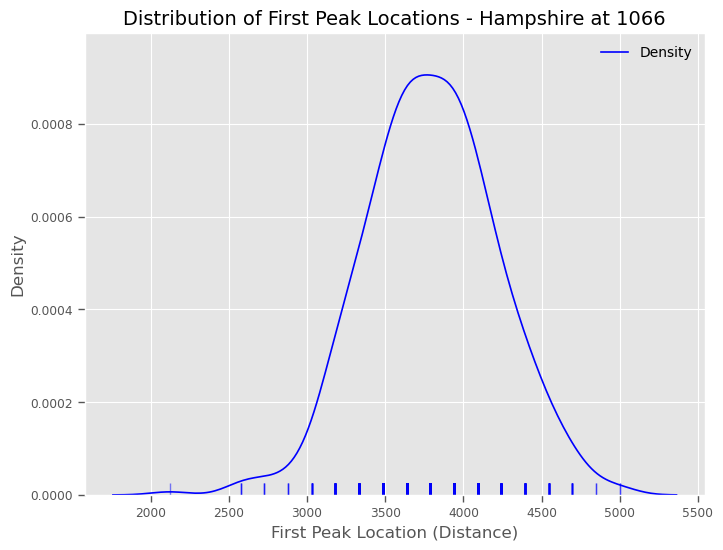
\includegraphics{analysis_files/figure-pdf/cell-41-output-1.png}

\subsubsection{Difference Distribution}\label{difference-distribution}

\paragraph{Figure S21: Distribution of First Peak Location Differences
between Angkor and
Hampshire}\label{figure-s21-distribution-of-first-peak-location-differences-between-angkor-and-hampshire}

\begin{Shaded}
\begin{Highlighting}[]
\CommentTok{\# Assuming \textasciigrave{}peaks\textasciigrave{} is your data}
\CommentTok{\# Plot density and rug plot}
\NormalTok{plt.figure(figsize}\OperatorTok{=}\NormalTok{(}\DecValTok{8}\NormalTok{, }\DecValTok{6}\NormalTok{))}
\NormalTok{sns.kdeplot(}
\NormalTok{    p\_pdd\_peaks\_hampshire }\OperatorTok{{-}}\NormalTok{ p\_pdd\_peaks\_angkor, }
\NormalTok{    color }\OperatorTok{=} \StringTok{\textquotesingle{}blue\textquotesingle{}}\NormalTok{, }
\NormalTok{    label }\OperatorTok{=} \StringTok{"Density"}\NormalTok{)}
\NormalTok{sns.rugplot(}
\NormalTok{    p\_pdd\_peaks\_hampshire }\OperatorTok{{-}}\NormalTok{ p\_pdd\_peaks\_angkor, }
\NormalTok{    color }\OperatorTok{=} \StringTok{\textquotesingle{}blue\textquotesingle{}}\NormalTok{, }
\NormalTok{    alpha }\OperatorTok{=} \FloatTok{0.5}\NormalTok{)}

\CommentTok{\# Add labels and title}
\NormalTok{plt.xlabel(}\StringTok{"First Peak Location Difference"}\NormalTok{)}
\NormalTok{plt.ylabel(}\StringTok{"Density"}\NormalTok{)}
\NormalTok{plt.title(}\StringTok{"Distribution of First Peak Location Differences"}\NormalTok{)}
\NormalTok{plt.legend()}

\CommentTok{\# Show the plot}
\NormalTok{plt.show()}
\end{Highlighting}
\end{Shaded}

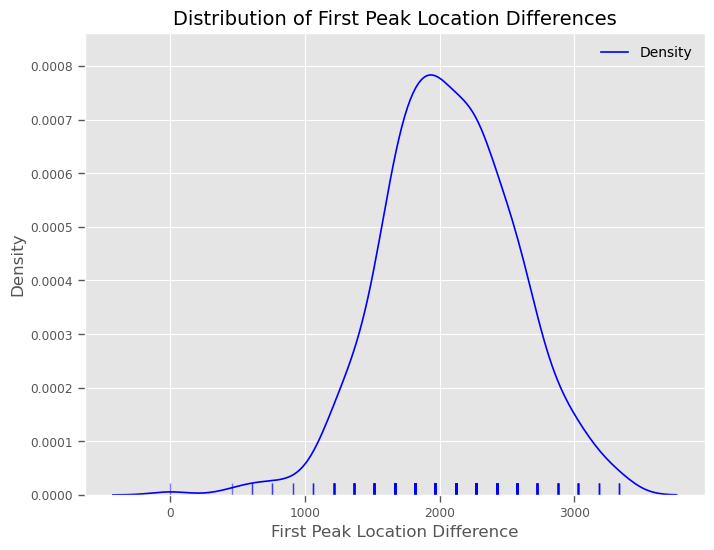
\includegraphics{analysis_files/figure-pdf/cell-42-output-1.png}

\begin{Shaded}
\begin{Highlighting}[]
\CommentTok{\# Convert to a Pandas DataFrame and use describe()}
\NormalTok{summary\_stats }\OperatorTok{=}\NormalTok{ pd.DataFrame(}
\NormalTok{    p\_pdd\_peaks\_hampshire }\OperatorTok{/}\NormalTok{ p\_pdd\_peaks\_angkor, }
\NormalTok{    columns }\OperatorTok{=}\NormalTok{ [}\StringTok{"Values"}\NormalTok{]}
\NormalTok{).describe()}

\CommentTok{\# Display the summary statistics}
\NormalTok{summary\_stats}
\end{Highlighting}
\end{Shaded}

\begin{longtable}[]{@{}ll@{}}
\toprule\noalign{}
& Values \\
\midrule\noalign{}
\endhead
\bottomrule\noalign{}
\endlastfoot
count & 500.000000 \\
mean & 2.256439 \\
std & 0.434235 \\
min & 1.000000 \\
25\% & 1.927198 \\
50\% & 2.181818 \\
75\% & 2.545455 \\
max & 3.750000 \\
\end{longtable}

\paragraph{Figure S22: Distribution of First Peal Location Ratios
between Angkor and
Hampshire}\label{figure-s22-distribution-of-first-peal-location-ratios-between-angkor-and-hampshire}

\begin{Shaded}
\begin{Highlighting}[]
\CommentTok{\# Assuming \textasciigrave{}peaks\textasciigrave{} is your data}
\CommentTok{\# Plot density and rug plot}
\NormalTok{plt.figure(figsize}\OperatorTok{=}\NormalTok{(}\DecValTok{8}\NormalTok{, }\DecValTok{6}\NormalTok{))}
\NormalTok{sns.kdeplot(}
\NormalTok{    p\_pdd\_peaks\_hampshire }\OperatorTok{/}\NormalTok{ p\_pdd\_peaks\_angkor, }
\NormalTok{    color }\OperatorTok{=} \StringTok{\textquotesingle{}blue\textquotesingle{}}\NormalTok{, }
\NormalTok{    label }\OperatorTok{=} \StringTok{"Density"}
\NormalTok{)}
\NormalTok{sns.rugplot(}
\NormalTok{    p\_pdd\_peaks\_hampshire }\OperatorTok{/}\NormalTok{ p\_pdd\_peaks\_angkor, }
\NormalTok{    color }\OperatorTok{=} \StringTok{\textquotesingle{}blue\textquotesingle{}}\NormalTok{, }
\NormalTok{    alpha }\OperatorTok{=} \FloatTok{0.5}
\NormalTok{)}

\CommentTok{\# Add labels and title}
\NormalTok{plt.xlabel(}\StringTok{"First Peak Location Ratio"}\NormalTok{)}
\NormalTok{plt.ylabel(}\StringTok{"Density"}\NormalTok{)}
\NormalTok{plt.title(}\StringTok{"Distribution of First Peak Location Ratios"}\NormalTok{)}
\NormalTok{plt.legend()}

\CommentTok{\# Show the plot}
\NormalTok{plt.show()}
\end{Highlighting}
\end{Shaded}

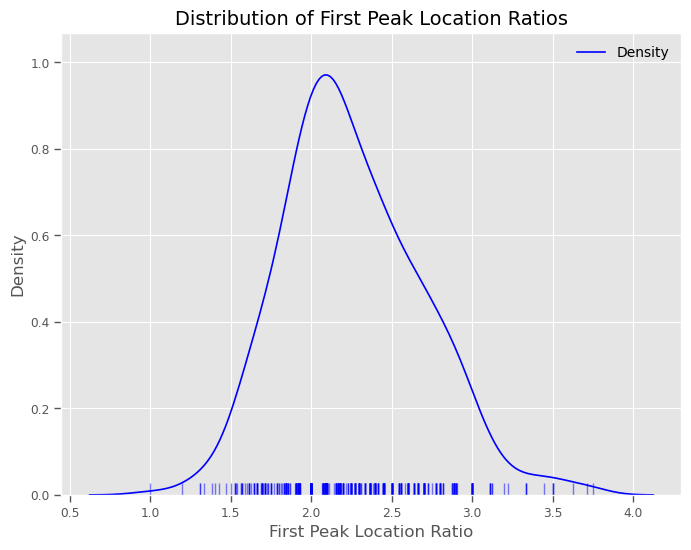
\includegraphics{analysis_files/figure-pdf/cell-44-output-1.png}

\subsection{Extended Analyses}\label{extended-analyses}

\begin{Shaded}
\begin{Highlighting}[]
\CommentTok{\# get unique list of counties}
\NormalTok{counties }\OperatorTok{=}\NormalTok{ doomsday\_places[}\StringTok{\textquotesingle{}County\textquotesingle{}}\NormalTok{].unique()}

\CommentTok{\# Ensure the Output directory exists}
\NormalTok{output\_dir }\OperatorTok{=} \StringTok{"../Output"}
\NormalTok{os.makedirs(output\_dir, exist\_ok}\OperatorTok{=}\VariableTok{True}\NormalTok{)}

\CommentTok{\# loop over it}
\ControlFlowTok{for}\NormalTok{ j }\KeywordTok{in}\NormalTok{ tqdm(counties, desc}\OperatorTok{=}\StringTok{"Processing Counties"}\NormalTok{):}
    \CommentTok{\# isolate j}
\NormalTok{    doomsday\_df }\OperatorTok{=}\NormalTok{ doomsday\_places[doomsday\_places[}\StringTok{\textquotesingle{}County\textquotesingle{}}\NormalTok{] }\OperatorTok{==}\NormalTok{ j]}

    \CommentTok{\# create list of points}
\NormalTok{    doomsday\_points }\OperatorTok{=}\NormalTok{ [}
\NormalTok{    clustering.Point(}
\NormalTok{        x}\OperatorTok{=}\NormalTok{row[}\StringTok{\textquotesingle{}easting\textquotesingle{}}\NormalTok{],}
\NormalTok{        y}\OperatorTok{=}\NormalTok{row[}\StringTok{\textquotesingle{}northing\textquotesingle{}}\NormalTok{],}
\NormalTok{        start\_distribution }\OperatorTok{=}\NormalTok{ ddelta(}\DecValTok{1066}\NormalTok{),}
\NormalTok{        end\_distribution }\OperatorTok{=}\NormalTok{ ddelta(}\DecValTok{1086}\NormalTok{)}
\NormalTok{    )}
    \ControlFlowTok{for}\NormalTok{ \_, row }\KeywordTok{in}\NormalTok{ doomsday\_df.iterrows()}
\NormalTok{    ]}

    \CommentTok{\# Define the time slices}
\NormalTok{    start\_time }\OperatorTok{=} \DecValTok{1066}
\NormalTok{    end\_time }\OperatorTok{=} \DecValTok{1086}
\NormalTok{    time\_interval }\OperatorTok{=} \DecValTok{5}
\NormalTok{    time\_slices }\OperatorTok{=}\NormalTok{ np.arange(start\_time, end\_time, time\_interval)}
\NormalTok{    time\_slices}

    \CommentTok{\# Get a bounding box for use later and to extract sensible distance limits}
\NormalTok{    x\_min, y\_min, x\_max, y\_max }\OperatorTok{=}\NormalTok{ get\_box(doomsday\_points)}
\NormalTok{    max\_distance }\OperatorTok{=}\NormalTok{ np.ceil(np.sqrt((x\_max }\OperatorTok{{-}}\NormalTok{ x\_min)}\OperatorTok{**}\DecValTok{2} \OperatorTok{+}\NormalTok{ (y\_max }\OperatorTok{{-}}\NormalTok{ y\_min)}\OperatorTok{**}\DecValTok{2}\NormalTok{))}

    \CommentTok{\# Run the Monte Carlo simulation to get an ensemble of probable }
    \CommentTok{\# lists of points included in each time slice.}
\NormalTok{    num\_iterations }\OperatorTok{=} \DecValTok{500}


    \CommentTok{\# set consistent pairwise bandwidth (binning of distances)}
\NormalTok{    use\_kde }\OperatorTok{=} \VariableTok{True}
\NormalTok{    pair\_bw }\OperatorTok{=} \VariableTok{None}
\NormalTok{    kde\_sample\_n }\OperatorTok{=} \DecValTok{50}
\NormalTok{    kde\_custom}\OperatorTok{=}\NormalTok{cuml\_kde}

    \CommentTok{\# Run the Monte Carlo simulation to get an ensemble of probable }
    \CommentTok{\# lists of points included in each time slice.}
\NormalTok{    simulations }\OperatorTok{=}\NormalTok{ clustering.mc\_samples(doomsday\_points, }
\NormalTok{                                        time\_slices}\OperatorTok{=}\NormalTok{time\_slices,  }
\NormalTok{                                        num\_iterations}\OperatorTok{=}\NormalTok{num\_iterations)}

    \CommentTok{\# set consistent pairwise bandwidth (binning of distances)}
    \CommentTok{\# same as before with Angkor data}
    \CommentTok{\# Produce pairwise distances to explore clustering structure}
\NormalTok{    pairwise\_density, support }\OperatorTok{=}\NormalTok{ clustering.temporal\_pairwise(}
\NormalTok{        simulations, }
\NormalTok{        time\_slices, }
\NormalTok{        bw }\OperatorTok{=}\NormalTok{ pair\_bw, }
\NormalTok{        use\_kde }\OperatorTok{=}\NormalTok{ use\_kde, }
\NormalTok{        kde\_sample\_n }\OperatorTok{=}\NormalTok{ kde\_sample\_n,}
\NormalTok{        max\_distance }\OperatorTok{=}\NormalTok{ max\_distance,}
\NormalTok{        kde\_custom }\OperatorTok{=}\NormalTok{ kde\_custom}
\NormalTok{    )}
    
    \CommentTok{\# Get MC iterations for incorporating chronological uncertainty with BISE}
\NormalTok{    bise\_simulations }\OperatorTok{=}\NormalTok{ clustering.mc\_samples(}
\NormalTok{        doomsday\_points, }
\NormalTok{        time\_slices, }
\NormalTok{        num\_iterations}\OperatorTok{=}\NormalTok{num\_iterations,}
\NormalTok{        null\_model}\OperatorTok{=}\NormalTok{clustering.bise}
\NormalTok{    )}

    \CommentTok{\# Calulate the pairwise distances for the LISE sample}
\NormalTok{    bise\_pairwise\_density, bise\_support }\OperatorTok{=}\NormalTok{ clustering.temporal\_pairwise(}
\NormalTok{        bise\_simulations, }
\NormalTok{        time\_slices, }
\NormalTok{        bw }\OperatorTok{=}\NormalTok{ pair\_bw, }
\NormalTok{        use\_kde }\OperatorTok{=}\NormalTok{ use\_kde,}
\NormalTok{        kde\_sample\_n}\OperatorTok{=}\NormalTok{kde\_sample\_n, }
\NormalTok{        max\_distance }\OperatorTok{=}\NormalTok{ max\_distance,}
\NormalTok{        kde\_custom}\OperatorTok{=}\NormalTok{kde\_custom}
\NormalTok{    )}

    \CommentTok{\# Calculate the p{-}values for density differences between the observed points and }
    \CommentTok{\# the simulated CSR baseline per distance and temporal slice}
\NormalTok{    p\_diff\_array, diff\_array }\OperatorTok{=}\NormalTok{ clustering.p\_diff(}
\NormalTok{        pairwise\_density, }
\NormalTok{        bise\_pairwise\_density}
\NormalTok{    )}

    \CommentTok{\#from chronocluster.utils import plot\_pdd}
\NormalTok{    time\_slice\_idx }\OperatorTok{=}\NormalTok{ np.where(time\_slices }\OperatorTok{==} \DecValTok{1066}\NormalTok{)[}\DecValTok{0}\NormalTok{][}\DecValTok{0}\NormalTok{]}

    \CommentTok{\# List of density arrays}
\NormalTok{    density\_arrays }\OperatorTok{=}\NormalTok{ [diff\_array]}

    \CommentTok{\# Generate the plot and get the figure and axis objects}
\NormalTok{    fig, ax }\OperatorTok{=}\NormalTok{ plot\_pdd(}
\NormalTok{        time\_slices}\OperatorTok{=}\NormalTok{time\_slices,}
\NormalTok{        time\_slice\_idx}\OperatorTok{=}\NormalTok{time\_slice\_idx,}
\NormalTok{        support}\OperatorTok{=}\NormalTok{support,}
\NormalTok{        density\_arrays}\OperatorTok{=}\NormalTok{density\_arrays,}
\NormalTok{        quantiles}\OperatorTok{=}\NormalTok{[}\FloatTok{0.025}\NormalTok{, }\FloatTok{0.975}\NormalTok{],}
\NormalTok{        density\_names}\OperatorTok{=}\NormalTok{[}\StringTok{"Diff Array"}\NormalTok{],}
\NormalTok{        colors}\OperatorTok{=}\NormalTok{[}\StringTok{"blue"}\NormalTok{]}
\NormalTok{    )}

    \CommentTok{\# Add a horizontal line at y=0}
\NormalTok{    ax.axhline(y}\OperatorTok{=}\DecValTok{0}\NormalTok{, color}\OperatorTok{=}\StringTok{\textquotesingle{}red\textquotesingle{}}\NormalTok{, linestyle}\OperatorTok{=}\StringTok{\textquotesingle{}{-}{-}\textquotesingle{}}\NormalTok{, linewidth}\OperatorTok{=}\FloatTok{1.5}\NormalTok{)}

    \CommentTok{\# Save the plot to the Output directory}
\NormalTok{    output\_path }\OperatorTok{=}\NormalTok{ os.path.join(output\_dir, }\SpecialStringTok{f"pdd\_}\SpecialCharTok{\{}\NormalTok{j}\SpecialCharTok{\}}\SpecialStringTok{.png"}\NormalTok{)}

\NormalTok{    plt.savefig(output\_path, dpi}\OperatorTok{=}\DecValTok{300}\NormalTok{, bbox\_inches}\OperatorTok{=}\StringTok{\textquotesingle{}tight\textquotesingle{}}\NormalTok{)}

    \CommentTok{\# Close the plot to free memory}
\NormalTok{    plt.close(fig)}
\end{Highlighting}
\end{Shaded}




\end{document}
